\documentclass[]{article}
\usepackage{lmodern}
\usepackage{amssymb,amsmath}
\usepackage{ifxetex,ifluatex}
\usepackage{fixltx2e} % provides \textsubscript
\ifnum 0\ifxetex 1\fi\ifluatex 1\fi=0 % if pdftex
  \usepackage[T1]{fontenc}
  \usepackage[utf8]{inputenc}
\else % if luatex or xelatex
  \ifxetex
    \usepackage{mathspec}
  \else
    \usepackage{fontspec}
  \fi
  \defaultfontfeatures{Ligatures=TeX,Scale=MatchLowercase}
\fi
% use upquote if available, for straight quotes in verbatim environments
\IfFileExists{upquote.sty}{\usepackage{upquote}}{}
% use microtype if available
\IfFileExists{microtype.sty}{%
\usepackage{microtype}
\UseMicrotypeSet[protrusion]{basicmath} % disable protrusion for tt fonts
}{}
\usepackage[margin=1in]{geometry}
\usepackage{hyperref}
\hypersetup{unicode=true,
            pdftitle={Laborator 1},
            pdfborder={0 0 0},
            breaklinks=true}
\urlstyle{same}  % don't use monospace font for urls
\usepackage{natbib}
\bibliographystyle{plainnat}
\usepackage{color}
\usepackage{fancyvrb}
\newcommand{\VerbBar}{|}
\newcommand{\VERB}{\Verb[commandchars=\\\{\}]}
\DefineVerbatimEnvironment{Highlighting}{Verbatim}{commandchars=\\\{\}}
% Add ',fontsize=\small' for more characters per line
\usepackage{framed}
\definecolor{shadecolor}{RGB}{248,248,248}
\newenvironment{Shaded}{\begin{snugshade}}{\end{snugshade}}
\newcommand{\AlertTok}[1]{\textcolor[rgb]{0.94,0.16,0.16}{#1}}
\newcommand{\AnnotationTok}[1]{\textcolor[rgb]{0.56,0.35,0.01}{\textbf{\textit{#1}}}}
\newcommand{\AttributeTok}[1]{\textcolor[rgb]{0.77,0.63,0.00}{#1}}
\newcommand{\BaseNTok}[1]{\textcolor[rgb]{0.00,0.00,0.81}{#1}}
\newcommand{\BuiltInTok}[1]{#1}
\newcommand{\CharTok}[1]{\textcolor[rgb]{0.31,0.60,0.02}{#1}}
\newcommand{\CommentTok}[1]{\textcolor[rgb]{0.56,0.35,0.01}{\textit{#1}}}
\newcommand{\CommentVarTok}[1]{\textcolor[rgb]{0.56,0.35,0.01}{\textbf{\textit{#1}}}}
\newcommand{\ConstantTok}[1]{\textcolor[rgb]{0.00,0.00,0.00}{#1}}
\newcommand{\ControlFlowTok}[1]{\textcolor[rgb]{0.13,0.29,0.53}{\textbf{#1}}}
\newcommand{\DataTypeTok}[1]{\textcolor[rgb]{0.13,0.29,0.53}{#1}}
\newcommand{\DecValTok}[1]{\textcolor[rgb]{0.00,0.00,0.81}{#1}}
\newcommand{\DocumentationTok}[1]{\textcolor[rgb]{0.56,0.35,0.01}{\textbf{\textit{#1}}}}
\newcommand{\ErrorTok}[1]{\textcolor[rgb]{0.64,0.00,0.00}{\textbf{#1}}}
\newcommand{\ExtensionTok}[1]{#1}
\newcommand{\FloatTok}[1]{\textcolor[rgb]{0.00,0.00,0.81}{#1}}
\newcommand{\FunctionTok}[1]{\textcolor[rgb]{0.00,0.00,0.00}{#1}}
\newcommand{\ImportTok}[1]{#1}
\newcommand{\InformationTok}[1]{\textcolor[rgb]{0.56,0.35,0.01}{\textbf{\textit{#1}}}}
\newcommand{\KeywordTok}[1]{\textcolor[rgb]{0.13,0.29,0.53}{\textbf{#1}}}
\newcommand{\NormalTok}[1]{#1}
\newcommand{\OperatorTok}[1]{\textcolor[rgb]{0.81,0.36,0.00}{\textbf{#1}}}
\newcommand{\OtherTok}[1]{\textcolor[rgb]{0.56,0.35,0.01}{#1}}
\newcommand{\PreprocessorTok}[1]{\textcolor[rgb]{0.56,0.35,0.01}{\textit{#1}}}
\newcommand{\RegionMarkerTok}[1]{#1}
\newcommand{\SpecialCharTok}[1]{\textcolor[rgb]{0.00,0.00,0.00}{#1}}
\newcommand{\SpecialStringTok}[1]{\textcolor[rgb]{0.31,0.60,0.02}{#1}}
\newcommand{\StringTok}[1]{\textcolor[rgb]{0.31,0.60,0.02}{#1}}
\newcommand{\VariableTok}[1]{\textcolor[rgb]{0.00,0.00,0.00}{#1}}
\newcommand{\VerbatimStringTok}[1]{\textcolor[rgb]{0.31,0.60,0.02}{#1}}
\newcommand{\WarningTok}[1]{\textcolor[rgb]{0.56,0.35,0.01}{\textbf{\textit{#1}}}}
\usepackage{longtable,booktabs}
\usepackage{graphicx,grffile}
\makeatletter
\def\maxwidth{\ifdim\Gin@nat@width>\linewidth\linewidth\else\Gin@nat@width\fi}
\def\maxheight{\ifdim\Gin@nat@height>\textheight\textheight\else\Gin@nat@height\fi}
\makeatother
% Scale images if necessary, so that they will not overflow the page
% margins by default, and it is still possible to overwrite the defaults
% using explicit options in \includegraphics[width, height, ...]{}
\setkeys{Gin}{width=\maxwidth,height=\maxheight,keepaspectratio}
\IfFileExists{parskip.sty}{%
\usepackage{parskip}
}{% else
\setlength{\parindent}{0pt}
\setlength{\parskip}{6pt plus 2pt minus 1pt}
}
\setlength{\emergencystretch}{3em}  % prevent overfull lines
\providecommand{\tightlist}{%
  \setlength{\itemsep}{0pt}\setlength{\parskip}{0pt}}
\setcounter{secnumdepth}{5}
% Redefines (sub)paragraphs to behave more like sections
\ifx\paragraph\undefined\else
\let\oldparagraph\paragraph
\renewcommand{\paragraph}[1]{\oldparagraph{#1}\mbox{}}
\fi
\ifx\subparagraph\undefined\else
\let\oldsubparagraph\subparagraph
\renewcommand{\subparagraph}[1]{\oldsubparagraph{#1}\mbox{}}
\fi

%%% Use protect on footnotes to avoid problems with footnotes in titles
\let\rmarkdownfootnote\footnote%
\def\footnote{\protect\rmarkdownfootnote}

%%% Change title format to be more compact
\usepackage{titling}

% Create subtitle command for use in maketitle
\providecommand{\subtitle}[1]{
  \posttitle{
    \begin{center}\large#1\end{center}
    }
}

\setlength{\droptitle}{-2em}

  \title{Laborator 1}
    \pretitle{\vspace{\droptitle}\centering\huge}
  \posttitle{\par}
  \subtitle{Introducere în R}
  \author{}
    \preauthor{}\postauthor{}
    \date{}
    \predate{}\postdate{}
  
\usepackage{booktabs}
\usepackage{longtable}
\usepackage{framed,color}
\definecolor{shadecolor}{RGB}{248, 248, 248}
\definecolor{shadecolor1}{RGB}{216,225,235}
\definecolor{framecolor}{RGB}{16,111,124}%108,123,13

%\definecolor{shadecolor}{RGB}{226, 255, 241}
% \definecolor{shadecolor1}{RGB}{217,225,199}
% \definecolor{framecolor}{RGB}{60,179,113}

%%%%%%%%%%%%%%%%%%%%%%
\ifxetex
  \usepackage{letltxmacro}
  \setlength{\XeTeXLinkMargin}{1pt}
  \LetLtxMacro\SavedIncludeGraphics\includegraphics
  \def\includegraphics#1#{% #1 catches optional stuff (star/opt. arg.)
    \IncludeGraphicsAux{#1}%
  }%
  \newcommand*{\IncludeGraphicsAux}[2]{%
    \XeTeXLinkBox{%
      \SavedIncludeGraphics#1{#2}%
    }%
  }%
\fi

\newenvironment{frshaded*}{%
  \def\FrameCommand{\fboxrule=\FrameRule\fboxsep=\FrameSep \fcolorbox{framecolor}{shadecolor1}}%
  \MakeFramed {\advance\hsize-\width \FrameRestore}}%
{\endMakeFramed}

\newenvironment{rmdblock}[1]
  {\begin{frshaded*}
  \begin{itemize}
  \renewcommand{\labelitemi}{
    \raisebox{-.7\height}[0pt][0pt]{
      {\setkeys{Gin}{width=2em,keepaspectratio}\includegraphics{images/icons/#1}}
    }
  }
  \item
  }
  {
  \end{itemize}
  \end{frshaded*}
  }
  
%%%%%%%%%%%%%%%
% definitions.
% -------------------
\usepackage{marginnote}
% \renewcommand*{\marginnotevadjust}{40pt}
% \renewcommand{\marginnotevadjust}{0pt}
% \renewcommand{\marginfont}{\noindent\rule{0pt}{0.7\baselineskip}\tiny}

\newtheorem{proposition}{Proposition}[section]
\newtheorem{lemma}[proposition]{Lemma}
\newtheorem{corollary}[proposition]{Corollary}
\newtheorem{theorem}[proposition]{Theorem}

\newcounter{exo}[section]
\newcommand{\enonce}[2]{\refstepcounter{proposition}\hypertarget{exo:#1}{}\label{exo:#1}{\scriptsize\;\textbf{Ex.}~\ref{exo:#1}}}

\reversemarginpar
\setlength{\marginparwidth}{1.2cm}
% 
% \newcommand{\enonce}[2]{\refstepcounter{proposition}\hypertarget{exo:#1}{}\label{exo:#1}{\noindent\color{black}\normalsize\bf Exercice \ref{exo:#1}}\ \  #2\vspace{1mm}\hrule\vspace{1mm} \color{black}\normalsize}


%%%%%%%%%%%%%%%

% \newenvironment{rmdcaution}
%   {\begin{rmdblock}{caution}}
%   {\end{rmdblock}}

% \newenvironment{rmdinsight}
%   {\begin{rmdblock}{insight}}
%   {\end{rmdblock}}

\newenvironment{rmdexercise}
  {\begin{rmdblock}{exercise}}
  {\end{rmdblock}}

% \newenvironment{rmdexercise_tex}
%   {\begin{rmdblock}{exercise}}
%   {\end{rmdblock}}
  
% \newenvironment{rmdtip}
%   {\begin{rmdblock}{tip}}
%   {\end{rmdblock}}


%%%%%%%%%%%%%%%%%%%%%%%%%%%%%%%%%%%%%%%%%%%%%%%%%%%%%%%%%%%%%%%%%%%%%%%%%%%%%%%%%%%%%%%%%%%%%%%%%%%%%%%%%%%%%%%%%%%%%
%%%%%%%%%%% For insight block %%%%%%%%%%%%%%%%%%%%%%%%%%
\definecolor{shadecolor_insight}{RGB}{223,240,216}
\definecolor{framecolor_insight}{RGB}{136,193,137}

%\definecolor{shadecolor_insight}{RGB}{217,225,199}
%\definecolor{framecolor_insight}{RGB}{60,179,113}

\newenvironment{frshaded_insight*}{%
  \def\FrameCommand{\fboxrule=\FrameRule\fboxsep=\FrameSep \fcolorbox{framecolor_insight}{shadecolor_insight}}%
  \MakeFramed {\advance\hsize-\width \FrameRestore}}%
{\endMakeFramed}

\newenvironment{rmdblock_insight}[1]
  {\begin{frshaded_insight*}
  \begin{itemize}
  \renewcommand{\labelitemi}{
    \raisebox{-.7\height}[0pt][0pt]{
      {\setkeys{Gin}{width=2em,keepaspectratio}\includegraphics{images/icons/#1}}
    }
  }
  \item
  }
  {
  \end{itemize}
  \end{frshaded_insight*}
  }

\newenvironment{rmdinsight}
  {\begin{rmdblock_insight}{insight}}
  {\end{rmdblock_insight}}

%%%%%%%%%%% For caution block %%%%%%%%%%%%%%%%%%%%%%%%%%
\definecolor{shadecolor_caution}{RGB}{250,250,250}
\definecolor{framecolor_caution}{RGB}{242,129,67}%193,75,34

\newenvironment{frshaded_caution*}{%
  \def\FrameCommand{\fboxrule=\FrameRule\fboxsep=\FrameSep \fcolorbox{framecolor_caution}{shadecolor_caution}}%
  \MakeFramed {\advance\hsize-\width \FrameRestore}}%
{\endMakeFramed}

\newenvironment{rmdblock_caution}[1]
  {\begin{frshaded_caution*}
  \begin{itemize}
  \renewcommand{\labelitemi}{
    \raisebox{-.7\height}[0pt][0pt]{
      {\setkeys{Gin}{width=2em,keepaspectratio}\includegraphics{images/icons/#1}}
    }
  }
  \item
  }
  {
  \end{itemize}
  \end{frshaded_caution*}
  }
  
\newenvironment{rmdcaution}
  {\begin{rmdblock_caution}{caution}}
  {\end{rmdblock_caution}}

%%%%%%%%%%% For tip block %%%%%%%%%%%%%%%%%%%%%%%%%%
\definecolor{shadecolor_tip}{RGB}{250,250,250}
\definecolor{framecolor_tip}{RGB}{33,153,195}

\newenvironment{frshaded_tip*}{%
  \def\FrameCommand{\fboxrule=\FrameRule\fboxsep=\FrameSep \fcolorbox{framecolor_tip}{shadecolor_tip}}%
  \MakeFramed {\advance\hsize-\width \FrameRestore}}%
{\endMakeFramed}

\newenvironment{rmdblock_tip}[1]
  {\begin{frshaded_tip*}
  \begin{itemize}
  \renewcommand{\labelitemi}{
    \raisebox{-.7\height}[0pt][0pt]{
      {\setkeys{Gin}{width=2em,keepaspectratio}\includegraphics{images/icons/#1}}
    }
  }
  \item
  }
  {
  \end{itemize}
  \end{frshaded_tip*}
  }
  
\newenvironment{rmdtip}
  {\begin{rmdblock_tip}{tip}}
  {\end{rmdblock_tip}}

%%%%%%%%%%%%%%%%%%%%%%%%%%%%%%%%%%%%%%%%%%%%%%%%%%%%%%%%%%%%%%%%%%%%%%%%%%%%%%%%%%%%%%%%%%%%%%%%%%%%%%%%%%%%%%%%%%%%%
\usepackage{subfigure}
\usepackage{booktabs}
\usepackage{slashbox}
\usepackage{color}
%%%%%%%%%%%%%%%%%%%%%%%%%%%%%%%%%%%%%%%%%
\definecolor{linkcol}{rgb}{0,0,0.4}
\definecolor{citecol}{rgb}{0.5,0,0}

% Change this to change the informations included in the pdf file
% \usepackage[pagebackref]{hyperref}
% \usepackage[verbose]{backref}
\usepackage[hyperpageref]{backref}
% \backrefsetup{verbose=false}
% \PassOptionsToPackage{pagebackref}{hyperref}
% See hyperref documentation for information on those parameters

\hypersetup
{
bookmarksopen=true,
pdftitle="Curs Statistica",
pdfauthor="Alexandru Amarioarei",
pdfsubject="Curs Statistica", %subject of the document
pdfmenubar=true, %menubar shown
pdfhighlight=/O, %effect of clicking on a link
colorlinks=true, %couleurs sur les liens hypertextes
pdfpagemode=None, %aucun mode de page
pdfpagelayout=SinglePage, %ouverture en simple page
pdffitwindow=true, %pages ouvertes entierement dans toute la fenetre
linkcolor=linkcol, %couleur des liens hypertextes internes
citecolor=citecol, %couleur des liens pour les citations
urlcolor=linkcol %couleur des liens pour les url
}


% set the back references
\renewcommand*{\backref}[1]{}
\renewcommand*{\backreftwosep}{ și~} % inserted between entries 
                              % in a list of two entries, 
                              % default is " and~".
\renewcommand*{\backreflastsep}{ și~} % inserted between the last 
                               % two entries of a list with more
                               % than two entries, default is ", and~".
\renewcommand*{\backrefalt}[4]{%
    \ifcase #1 (Necitat.)%
    \or        (Citat la pagina~#2.)%
    \else      (Citat la paginile~#2.)%
    \fi}

%%%%%%%%%%%%%%%%%%%%%%%%%%%%%%%%%%%%%%%%%%%%%%%%%%%%%%%%%%%%%%%%%%%%%%%%%%%%%%%%%%%%%%%%%%%%%%%%%%%%%%%%%%%%%%%%%%%%%
%CITEVA DEFINITII
\def\om{\omega}
\def\Om{\Omega}
\def\et{\eta}
\def\td{\tilde{\delta}}
\def\m{{\mu}}
\def\n{{\nu}}
\def\k{{\kappa}}
\def\l{{\lambda}}
\def\L{{\Lambda}}
\def\g{{\gamma}}
\def\a{{\alpha}}
\def\e{{\varepsilon}}
\def\b{{\beta}}
\def\G{{\Gamma}}
\def\d{{\delta}}
\def\D{{\Delta}}
\def\t{{\theta}}
\def\s{{\sigma}}
\def\S{{\Sigma}}
\def\z{{\zeta}}
\def\qed{\hfill\Box}
\def\ds{\displaystyle}
\def\mc{\mathcal}
%%%%%%%%%%%%%%%%%%%%%%%%%%%%%%%%%%%%%%%%%%%%%%%%%%%%%%%%%%%%%%%%%%%%%%%%%%%%%%%%%%%%%%%%%%%%%%%%%%%%%%%%%%%%%%%%%%%%%%
\def\1{{\mathbf 1}}
\def\CC{{\mathbb C}}
\def\VV{{\mathbb V}}
\def\RR{{\mathbb R}}
\def\QQ{{\mathbb Q}}
\def\ZZ{{\mathbb Z}}
\def\PP{{\mathbb P}}
\def\EE{{\mathbb E}}
\def\NN{{\mathbb N}}
\def\FF{{\mathbb F}}
%\def\SS{{\mathbb S}}
\def\MA{{\mathcal A}}
\def\MO{{\mathcal O}}
\def\MF{{\mathcal F}}
\def\ME{{\mathcal E}}
\def\MR{{\mathcal R}}
\def\MB{{\mathcal B}}
\def\MM{{\mathcal M}}
\def\MN{{\mathcal N}}
\def\MU{{\mathcal U}}
\def\MP{{\mathcal P}}
\def\MS{{\mathcal S}}
\def\MBS{{\mathbf S}}
\def\MX{{\bm{ \mathscr X}}}

% independent sign
\newcommand\independent{\protect\mathpalette{\protect\independenT}{\perp}}
\def\independenT#1#2{\mathrel{\rlap{$#1#2$}\mkern2mu{#1#2}}}

\renewcommand\tablename{Tab.}
\renewcommand{\figurename}{Fig.}
\renewcommand\refname{Referințe}

%%%%%%%%%%%%%%%%%%%%%%%%%%%%%%%%%%%%%%%%%%%%%%%%%%%%%%%%%%%%%%%%%%%%%%%%%%%%%%%%%%%%%%%%%%%%%%%%%%%%%%%%%%%%%%%%%%%%%
%Header and Footer
\usepackage{fancyhdr}

\pagestyle{fancy}
\fancyhf{}
\rhead{Universitatea din Bucure\c sti\\ Facultatea de Matematic\u a \c si Informatic\u a}
% \lhead{\textit{Curs}: Tehnici alternative în predarea matematicii (2018)\\ \textit{Instructori}: A. Am\u arioarei, M. Patriche}
\lhead{\textit{Curs}: Statistică (2019-2020)\\ \textit{Instructori}: A. Am\u arioarei, S. Cojocea}
\rfoot{Pagina \thepage}
\lfoot{Grupele: 301, 311, 321}
%%%%%%%%%%%%%%%%%%%%%%%%%%%%%%%%%%%%%%%
%%%%%%%%%%%%%%%%%%%%%%%%%%%%%%%%%%%%%%%
\usepackage{pifont}% http://ctan.org/pkg/pifont
\newcommand{\cmark}{\ding{51}}%
\newcommand{\xmark}{\ding{55}}%
\usepackage{booktabs}
\usepackage{longtable}
\usepackage{array}
\usepackage{multirow}
\usepackage{wrapfig}
\usepackage{float}
\usepackage{colortbl}
\usepackage{pdflscape}
\usepackage{tabu}
\usepackage{threeparttable}
\usepackage{threeparttablex}
\usepackage[normalem]{ulem}
\usepackage{makecell}
\usepackage{xcolor}

\begin{document}
\maketitle

%%%%%%%%%%%%%%%%%%%%%%%%
\thispagestyle{fancy}

Obiectivul acestui laborator este de a prezenta o scurtă introducere în
programul \href{https://cran.r-project.org/}{R} (cu ajutorul interfeței
grafice \href{https://www.rstudio.com/}{RStudio}). O descriere detaliată
a acestui program precum și versiunile disponibile pentru descărcat se
găsesc pe site-ul
\href{http://www.r-project.org}{\texttt{www.r-project.org}}. Pentru mai
multe detalii se pot consulta \citep[\citet{Matloff2011}]{Davies2016}.

\hypertarget{introducere}{%
\section{Introducere}\label{introducere}}

Programul \texttt{R} este un program \textbf{gratuit} destinat, cu
precădere, analizei statistice și prezintă o serie de avantaje:

\begin{itemize}
\tightlist
\item
  rulează aproape pe toate platformele și sistemele de operare
\item
  permite folosirea metodelor statistice clasice cu ajutorul unor
  funcții predefinite
\item
  este adoptat ca limbaj de analiză statistică în majoritatea domeniilor
  aplicate
\item
  prezintă capabilități grafice deosebite
\item
  permite utilizarea tehnicilor statistice de ultimă oră prin
  intermediul pachetelor dezvoltate de comunitate (în prezent sunt mai
  mult de 10000 de pachete)
\item
  are o comunitate foarte activă și în continuă creștere
\end{itemize}

\begin{figure}

{\centering 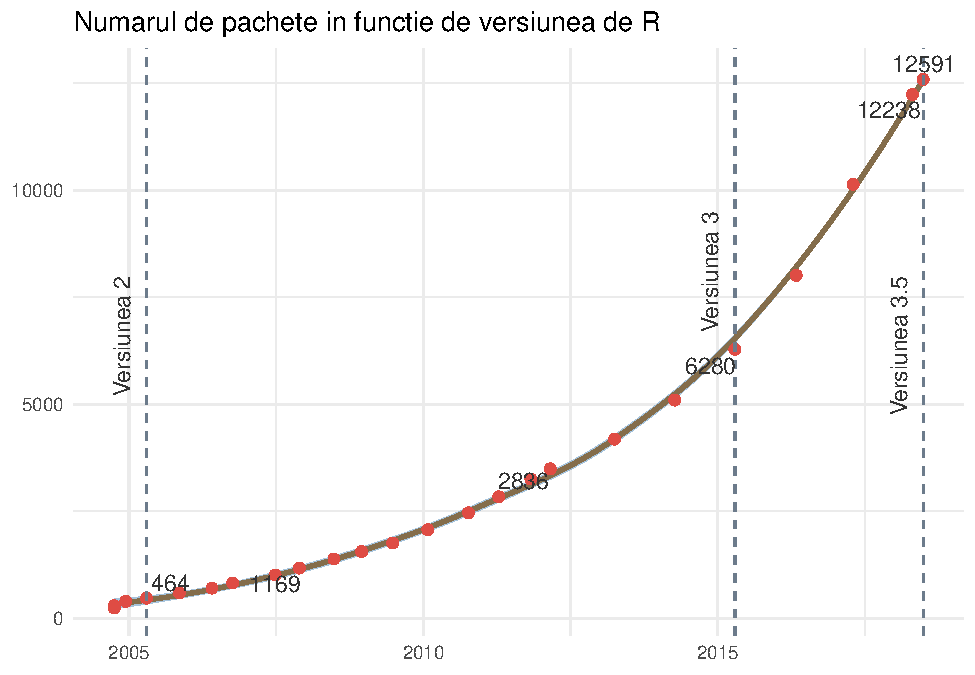
\includegraphics[width=0.8\linewidth]{Lab1_files/figure-latex/unnamed-chunk-3-1} 

}

\caption{Numarul de pachete din R}\label{fig:unnamed-chunk-3}
\end{figure}

\hypertarget{interfaux21ba-rstudio}{%
\subsection{\texorpdfstring{Interfața
\texttt{RStudio}}{Interfața RStudio}}\label{interfaux21ba-rstudio}}

Interfața RStudio (vezi Figura 1) este compusă din patru ferestre:

\begin{itemize}
\tightlist
\item
  \emph{Fereastra de editare} (stânga sus): în această fereastră apar
  fișierele, de tip \texttt{script}, în care utilizatorul dezvoltă
  propriile funcții ori script-uri.\\
\item
  \emph{Fereastra de comandă} sau \emph{consola} (stânga jos): în
  această fereastră sunt executate comenzile R
\item
  \emph{Fereastra cu spațiul de lucru/istoricul} (dreapta sus): conține
  obiectele definite în memorie și istoricul comenzilor folosite
\item
  \emph{Fereastra de explorare} (dreapta jos): în această fereastră ne
  putem deplasa în interiorul repertoriului (tab-ul \emph{Files}), putem
  vedea graficele trasate (tab-ul \emph{Plots}) dar și pachetele
  instalate (tab-ul \emph{Packages}). De asemenea, tot în această
  fereastră putem să și căutăm documentația despre diferite funcții,
  folosind fereastra de ajutor (tab-ul \emph{Help}).
\end{itemize}

\begin{figure}

{\centering 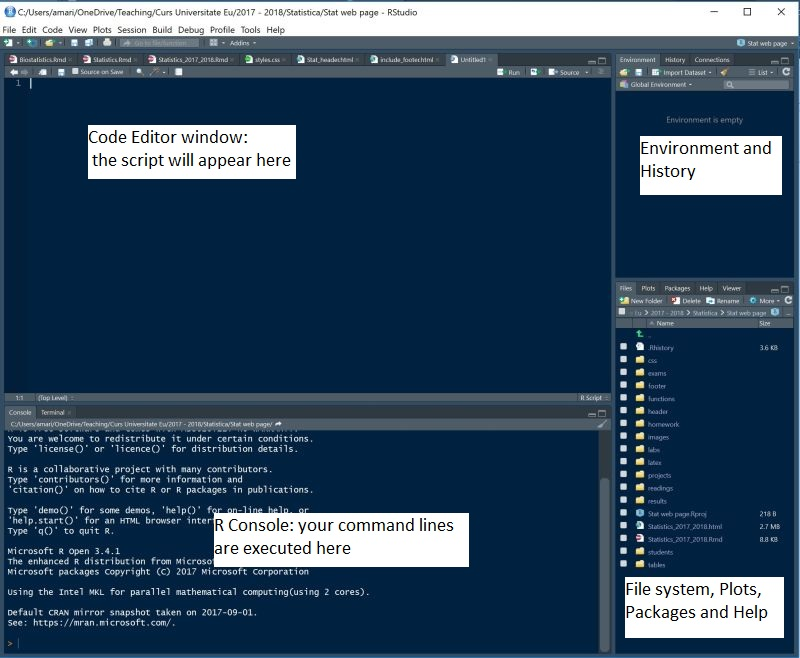
\includegraphics[width=0.8\linewidth]{images/Lab1/RStudio3} 

}

\caption{Interfata RStudio}\label{fig:unnamed-chunk-4}
\end{figure}

\hypertarget{pachetele-ajutux103toare}{%
\subsection{Pachetele ajutătoare}\label{pachetele-ajutux103toare}}

Pe lângă diferitele pachete conținute în versiunea de bază a programului
\texttt{R} se mai pot instala și pachete suplimentare. Pentru a instala
un pachet suplimentar se apelează comanda:

\begin{Shaded}
\begin{Highlighting}[]
\KeywordTok{install.packages}\NormalTok{(}\StringTok{"nume pachet"}\NormalTok{)}
\end{Highlighting}
\end{Shaded}

Odată ce pachetul este instalat, pentru a încărca pachetul, și prin
urmare funcțiile disponibile în acesta, se apelează comanda:

\begin{Shaded}
\begin{Highlighting}[]
\KeywordTok{library}\NormalTok{(}\StringTok{"nume pachet"}\NormalTok{)}
\end{Highlighting}
\end{Shaded}

Instalarea unui pachet se face o singură dată dar încărcarea acestuia
trebuie făcută de fiecare dată când lansăm o sesiune nouă.

\hypertarget{primele-comenzi-uxeen-r}{%
\section{\texorpdfstring{Primele comenzi în
\texttt{R}}{Primele comenzi în R}}\label{primele-comenzi-uxeen-r}}

\hypertarget{calcul-elementar}{%
\subsection{Calcul elementar}\label{calcul-elementar}}

Programul \texttt{R} poate fi folosit și pe post de calculator (mai
avansat). De exemplu putem face calcule elementare

\begin{Shaded}
\begin{Highlighting}[]
\DecValTok{5} \OperatorTok{-}\StringTok{ }\DecValTok{1} \OperatorTok{+}\StringTok{ }\DecValTok{10}
\NormalTok{[}\DecValTok{1}\NormalTok{] }\DecValTok{14}
\DecValTok{7} \OperatorTok{*}\StringTok{ }\DecValTok{10} \OperatorTok{/}\StringTok{ }\DecValTok{2}
\NormalTok{[}\DecValTok{1}\NormalTok{] }\DecValTok{35}
\KeywordTok{exp}\NormalTok{(}\OperatorTok{-}\FloatTok{2.19}\NormalTok{)}
\NormalTok{[}\DecValTok{1}\NormalTok{] }\FloatTok{0.1119167}
\NormalTok{pi}
\NormalTok{[}\DecValTok{1}\NormalTok{] }\FloatTok{3.141593}
\KeywordTok{sin}\NormalTok{(}\DecValTok{2} \OperatorTok{*}\StringTok{ }\NormalTok{pi}\OperatorTok{/}\DecValTok{3}\NormalTok{)}
\NormalTok{[}\DecValTok{1}\NormalTok{] }\FloatTok{0.8660254}
\end{Highlighting}
\end{Shaded}

De asemenea, rezultatele pot fi stocate într-o variabilă

\begin{Shaded}
\begin{Highlighting}[]
\NormalTok{a =}\StringTok{ }\NormalTok{(}\DecValTok{1}\OperatorTok{+}\KeywordTok{sqrt}\NormalTok{(}\DecValTok{5}\NormalTok{)}\OperatorTok{/}\DecValTok{2}\NormalTok{)}\OperatorTok{/}\DecValTok{2}
\end{Highlighting}
\end{Shaded}

păstrată în memorie (\texttt{a} apare în fereastra de lucru -
\texttt{Environment}) și care poate fi reutilizată ulterior

\begin{Shaded}
\begin{Highlighting}[]
\NormalTok{asq =}\StringTok{ }\KeywordTok{sqrt}\NormalTok{(a)}
\NormalTok{asq}
\NormalTok{[}\DecValTok{1}\NormalTok{] }\FloatTok{1.029086}
\end{Highlighting}
\end{Shaded}

Operațiile binare în \texttt{R} sunt date în tabelul de mai jos:

\begin{longtable}[]{@{}ll@{}}
\caption{Operatii binare in R}\tabularnewline
\toprule
Operatorul & Descriere\tabularnewline
\midrule
\endfirsthead
\toprule
Operatorul & Descriere\tabularnewline
\midrule
\endhead
\texttt{+} & Adunare\tabularnewline
\texttt{-} & Scădere\tabularnewline
\texttt{*} & Înmulțire\tabularnewline
\texttt{/} & Împărțire\tabularnewline
\texttt{\^{}} or \texttt{**} & Exponențiere\tabularnewline
\texttt{\%/\%} & Câtul împărțirii\tabularnewline
\texttt{\%\%} & Restul împărțirii\tabularnewline
\bottomrule
\end{longtable}

Pentru a șterge toate variabilele din memorie trebuie să folosim comanda
următoare (funcția \texttt{ls()} listează numele obiectelor din memorie
iar comanda \texttt{rm()} șterge obiectele; de asemenea se poate folosi
și comanda \texttt{ls.str()} pentru a lista obiectele împreună cu o
scurtă descriere a lor)

\begin{Shaded}
\begin{Highlighting}[]
\KeywordTok{ls.str}\NormalTok{()}
\KeywordTok{rm}\NormalTok{(}\DataTypeTok{list =} \KeywordTok{ls}\NormalTok{())}
\end{Highlighting}
\end{Shaded}

\hypertarget{folosirea-documentaux21biei}{%
\subsection{Folosirea documentației}\label{folosirea-documentaux21biei}}

Funcția \texttt{help()} și operatorul de ajutor \texttt{?} ne permite
accesul la paginile de documentația pentru funcțiile, seturile de date
și alte obiecte din R. Pentru a accesa documentația pentru funcția
standard \texttt{mean()} putem să folosim comanda \texttt{help(mean)}
sau \texttt{?mean} în consolă. Pentru a accesa documentația unei funcții
dintr-un pachet care nu este în prezent încărcat (dar este instalat)
trebuie să adăugăm în plus numele pachetului, de exemplu
\texttt{help(rlm,\ package\ =\ "MASS")} iar pentru a accesa documentația
întregului pachet putem folosi comanda
\texttt{help(package\ =\ "MASS")}.

O altă funcție de căutare des utilizată, în special în situația în care
nu știm cu exactitate numele obiectului pe care îl căutăm, este funcția
\texttt{apropos()}. Aceasta permite căutarea obiectelor (inclusiv
funcții), disponibile în pachetele încărcate în sesiunea curentă, după
un șir de caractere specificat (se pot folosi și expresii regulate). De
exemplu dacă apelăm \texttt{apropos("mean")} vom obține toate funcțiile
care conțin șirul de caractere \emph{mean}.

\begin{Shaded}
\begin{Highlighting}[]
\KeywordTok{apropos}\NormalTok{(}\StringTok{"mean"}\NormalTok{) }\CommentTok{# functii care contin mean}
\NormalTok{ [}\DecValTok{1}\NormalTok{] }\StringTok{".colMeans"}      \StringTok{".rowMeans"}      \StringTok{"colMeans"}       \StringTok{"kmeans"}        
\NormalTok{ [}\DecValTok{5}\NormalTok{] }\StringTok{"mean"}           \StringTok{"mean.Date"}      \StringTok{"mean.default"}   \StringTok{"mean.difftime"} 
\NormalTok{ [}\DecValTok{9}\NormalTok{] }\StringTok{"mean.POSIXct"}   \StringTok{"mean.POSIXlt"}   \StringTok{"mean_cl_boot"}   \StringTok{"mean_cl_normal"}
\NormalTok{[}\DecValTok{13}\NormalTok{] }\StringTok{"mean_sdl"}       \StringTok{"mean_se"}        \StringTok{"rowMeans"}       \StringTok{"weighted.mean"} 

\KeywordTok{apropos}\NormalTok{(}\StringTok{"^mean"}\NormalTok{) }\CommentTok{# functii care incep cu mean}
\NormalTok{ [}\DecValTok{1}\NormalTok{] }\StringTok{"mean"}           \StringTok{"mean.Date"}      \StringTok{"mean.default"}   \StringTok{"mean.difftime"} 
\NormalTok{ [}\DecValTok{5}\NormalTok{] }\StringTok{"mean.POSIXct"}   \StringTok{"mean.POSIXlt"}   \StringTok{"mean_cl_boot"}   \StringTok{"mean_cl_normal"}
\NormalTok{ [}\DecValTok{9}\NormalTok{] }\StringTok{"mean_sdl"}       \StringTok{"mean_se"}       
\end{Highlighting}
\end{Shaded}

Următorul tabel prezintă funcțiile de ajutor, cel mai des utilizate:

\begin{longtable}[]{@{}ll@{}}
\caption{Functii folosite pentru ajutor}\tabularnewline
\toprule
\begin{minipage}[b]{0.42\columnwidth}\raggedright
Funcție\strut
\end{minipage} & \begin{minipage}[b]{0.52\columnwidth}\raggedright
Acțiune\strut
\end{minipage}\tabularnewline
\midrule
\endfirsthead
\toprule
\begin{minipage}[b]{0.42\columnwidth}\raggedright
Funcție\strut
\end{minipage} & \begin{minipage}[b]{0.52\columnwidth}\raggedright
Acțiune\strut
\end{minipage}\tabularnewline
\midrule
\endhead
\begin{minipage}[t]{0.42\columnwidth}\raggedright
\texttt{help.start()}\strut
\end{minipage} & \begin{minipage}[t]{0.52\columnwidth}\raggedright
Modul de ajutor general\strut
\end{minipage}\tabularnewline
\begin{minipage}[t]{0.42\columnwidth}\raggedright
\texttt{help("nume")} sau \texttt{?nume}\strut
\end{minipage} & \begin{minipage}[t]{0.52\columnwidth}\raggedright
Documentație privind funcția \emph{nume} (ghilimelele sunt
opționale)\strut
\end{minipage}\tabularnewline
\begin{minipage}[t]{0.42\columnwidth}\raggedright
\texttt{help.search(nume)} sau \texttt{??nume}\strut
\end{minipage} & \begin{minipage}[t]{0.52\columnwidth}\raggedright
Caută sistemul de documentație pentru instanțe în care apare șirul de
caractere \emph{nume}\strut
\end{minipage}\tabularnewline
\begin{minipage}[t]{0.42\columnwidth}\raggedright
\texttt{example("nume")}\strut
\end{minipage} & \begin{minipage}[t]{0.52\columnwidth}\raggedright
Exemple de utilizare ale funcției \emph{nume}\strut
\end{minipage}\tabularnewline
\begin{minipage}[t]{0.42\columnwidth}\raggedright
\texttt{RSiteSearch("nume")}\strut
\end{minipage} & \begin{minipage}[t]{0.52\columnwidth}\raggedright
Caută șirul de caractere \emph{nume} în manualele online și în
arhivă\strut
\end{minipage}\tabularnewline
\begin{minipage}[t]{0.42\columnwidth}\raggedright
\texttt{apropos("nume",\ mode\ =\ "functions")}\strut
\end{minipage} & \begin{minipage}[t]{0.52\columnwidth}\raggedright
Listează toate funcțiile care conțin șirul \emph{nume} în numele
lor\strut
\end{minipage}\tabularnewline
\begin{minipage}[t]{0.42\columnwidth}\raggedright
\texttt{data()}\strut
\end{minipage} & \begin{minipage}[t]{0.52\columnwidth}\raggedright
Listează toate seturile de date disponibile în pachetele încărcate\strut
\end{minipage}\tabularnewline
\begin{minipage}[t]{0.42\columnwidth}\raggedright
\texttt{vignette()}\strut
\end{minipage} & \begin{minipage}[t]{0.52\columnwidth}\raggedright
Listează toate vinietele disponibile\strut
\end{minipage}\tabularnewline
\begin{minipage}[t]{0.42\columnwidth}\raggedright
\texttt{vignette("nume")}\strut
\end{minipage} & \begin{minipage}[t]{0.52\columnwidth}\raggedright
Afișează vinietele corespunzătoare topicului \emph{nume}\strut
\end{minipage}\tabularnewline
\bottomrule
\end{longtable}

Documentații online:

\begin{longtable}[]{@{}ll@{}}
\caption{O serie de link-uri utile}\tabularnewline
\toprule
\begin{minipage}[b]{0.32\columnwidth}\raggedright
CheatSheet\strut
\end{minipage} & \begin{minipage}[b]{0.62\columnwidth}\raggedright
Link\strut
\end{minipage}\tabularnewline
\midrule
\endfirsthead
\toprule
\begin{minipage}[b]{0.32\columnwidth}\raggedright
CheatSheet\strut
\end{minipage} & \begin{minipage}[b]{0.62\columnwidth}\raggedright
Link\strut
\end{minipage}\tabularnewline
\midrule
\endhead
\begin{minipage}[t]{0.32\columnwidth}\raggedright
R de bază\strut
\end{minipage} & \begin{minipage}[t]{0.62\columnwidth}\raggedright
\url{https://cran.r-project.org/doc/contrib/Short-refcard.pdf}\strut
\end{minipage}\tabularnewline
\begin{minipage}[t]{0.32\columnwidth}\raggedright
Noțiuni de R avansat\strut
\end{minipage} & \begin{minipage}[t]{0.62\columnwidth}\raggedright
\url{https://www.rstudio.com/wp-content/uploads/2016/02/advancedR.pdf}\strut
\end{minipage}\tabularnewline
\begin{minipage}[t]{0.32\columnwidth}\raggedright
Noțiuni de R de bază\strut
\end{minipage} & \begin{minipage}[t]{0.62\columnwidth}\raggedright
\url{http://github.com/rstudio/cheatsheets/raw/master/base-r.pdf}\strut
\end{minipage}\tabularnewline
\begin{minipage}[t]{0.32\columnwidth}\raggedright
Manipularea șirurilor de caractere\strut
\end{minipage} & \begin{minipage}[t]{0.62\columnwidth}\raggedright
\url{https://github.com/rstudio/cheatsheets/raw/master/strings.pdf}\strut
\end{minipage}\tabularnewline
\begin{minipage}[t]{0.32\columnwidth}\raggedright
Importarea datelor\strut
\end{minipage} & \begin{minipage}[t]{0.62\columnwidth}\raggedright
\url{https://github.com/rstudio/cheatsheets/raw/master/data-import.pdf}\strut
\end{minipage}\tabularnewline
\begin{minipage}[t]{0.32\columnwidth}\raggedright
Transformarea datelor\strut
\end{minipage} & \begin{minipage}[t]{0.62\columnwidth}\raggedright
\url{https://github.com/rstudio/cheatsheets/raw/master/data-import.pdf}\strut
\end{minipage}\tabularnewline
\begin{minipage}[t]{0.32\columnwidth}\raggedright
RStudio\strut
\end{minipage} & \begin{minipage}[t]{0.62\columnwidth}\raggedright
\url{https://github.com/rstudio/cheatsheets/raw/master/rstudio-ide.pdf}\strut
\end{minipage}\tabularnewline
\begin{minipage}[t]{0.32\columnwidth}\raggedright
Pachetul ggplot2\strut
\end{minipage} & \begin{minipage}[t]{0.62\columnwidth}\raggedright
\url{https://github.com/rstudio/cheatsheets/raw/master/data-visualization-2.1.pdf}\strut
\end{minipage}\tabularnewline
\begin{minipage}[t]{0.32\columnwidth}\raggedright
Pachetul RMarkdown\strut
\end{minipage} & \begin{minipage}[t]{0.62\columnwidth}\raggedright
\url{https://www.rstudio.com/wp-content/uploads/2015/03/rmarkdown-reference.pdf}\strut
\end{minipage}\tabularnewline
\bottomrule
\end{longtable}

\hypertarget{tipuri-ux219i-structuri-de-date}{%
\section{Tipuri și structuri de
date}\label{tipuri-ux219i-structuri-de-date}}

\texttt{R} are cinci tipuri de date principale (atomi), după cum
urmează:

\begin{itemize}
\tightlist
\item
  \textbf{character}: \texttt{"a"}, \texttt{"swc"}
\item
  \textbf{numeric}: \texttt{2}, \texttt{15.5}
\item
  \textbf{integer}: \texttt{2L} (sufix-ul \texttt{L} îi spune R-ului să
  stocheze numărul ca pe un întreg)
\item
  \textbf{logical}: \texttt{TRUE}, \texttt{FALSE}
\item
  \textbf{complex}: \texttt{1+4i} (numere complexe)
\end{itemize}

R pune la dispoziție mai multe funcții cu ajutorul cărora se pot examina
trăsăturile vectorilor sau a altor obiecte, cum ar fi de exemplu

\begin{itemize}
\tightlist
\item
  \texttt{class()} - ce tip de obiect este
\item
  \texttt{typeof()} - care este tipul de date al obiectului
\item
  \texttt{length()} - care este lungimea obiectului
\item
  \texttt{attributes()} - care sunt atributele obiectului (metadata)
\end{itemize}

\begin{Shaded}
\begin{Highlighting}[]
\CommentTok{# Exemplu}
\NormalTok{x <-}\StringTok{ "curs probabilitati si statistica"}
\KeywordTok{typeof}\NormalTok{(x)}
\NormalTok{[}\DecValTok{1}\NormalTok{] }\StringTok{"character"}
\KeywordTok{attributes}\NormalTok{(x)}
\OtherTok{NULL}

\NormalTok{y <-}\StringTok{ }\DecValTok{1}\OperatorTok{:}\DecValTok{10}
\NormalTok{y}
\NormalTok{ [}\DecValTok{1}\NormalTok{]  }\DecValTok{1}  \DecValTok{2}  \DecValTok{3}  \DecValTok{4}  \DecValTok{5}  \DecValTok{6}  \DecValTok{7}  \DecValTok{8}  \DecValTok{9} \DecValTok{10}
\KeywordTok{typeof}\NormalTok{(y)}
\NormalTok{[}\DecValTok{1}\NormalTok{] }\StringTok{"integer"}
\KeywordTok{length}\NormalTok{(y)}
\NormalTok{[}\DecValTok{1}\NormalTok{] }\DecValTok{10}

\NormalTok{z <-}\StringTok{ }\KeywordTok{as.numeric}\NormalTok{(y)}
\NormalTok{z}
\NormalTok{ [}\DecValTok{1}\NormalTok{]  }\DecValTok{1}  \DecValTok{2}  \DecValTok{3}  \DecValTok{4}  \DecValTok{5}  \DecValTok{6}  \DecValTok{7}  \DecValTok{8}  \DecValTok{9} \DecValTok{10}
\KeywordTok{typeof}\NormalTok{(z)}
\NormalTok{[}\DecValTok{1}\NormalTok{] }\StringTok{"double"}
\end{Highlighting}
\end{Shaded}

În limbajul \texttt{R} regăsim mai multe \textbf{structuri de date}.
Printre acestea enumerăm

\begin{itemize}
\tightlist
\item
  vectorii (structuri atomice)
\item
  listele
\item
  matricele
\item
  data frame
\item
  factori
\end{itemize}

\hypertarget{scalari-ux219i-vectori}{%
\subsection{Scalari și vectori}\label{scalari-ux219i-vectori}}

Cel mai de bază tip de obiect în R este vectorul. Una dintre regulile
principale ale vectorilor este că aceștia pot conține numai obiecte de
același tip, cu alte cuvinte putem avea doar vectori de tip caracter,
numeric, logic, etc.. În cazul în care încercăm să combinăm diferite
tipuri de date, acestea vor fi forțate la tipul cel mai flexibil.
Tipurile de la cel mai puțin la cele mai flexibile sunt: logice,
întregi, numerice și caractere.

\hypertarget{metode-de-construcux21bie-a-vectorilor}{%
\subsubsection{Metode de construcție a
vectorilor}\label{metode-de-construcux21bie-a-vectorilor}}

Putem crea vectori fără elemente (empty) cu ajutorul funcției
\texttt{vector()}, modul default este \emph{logical} dar acesta se poate
schimba în funcție de necesitate.

\begin{Shaded}
\begin{Highlighting}[]
\KeywordTok{vector}\NormalTok{() }\CommentTok{# vector logic gol}
\KeywordTok{logical}\NormalTok{(}\DecValTok{0}\NormalTok{)}
\KeywordTok{vector}\NormalTok{(}\StringTok{"character"}\NormalTok{, }\DataTypeTok{length =} \DecValTok{5}\NormalTok{) }\CommentTok{# vector de caractere cu 5 elemente}
\NormalTok{[}\DecValTok{1}\NormalTok{] }\StringTok{""} \StringTok{""} \StringTok{""} \StringTok{""} \StringTok{""}
\KeywordTok{character}\NormalTok{(}\DecValTok{5}\NormalTok{) }\CommentTok{# acelasi lucru dar in mod direct}
\NormalTok{[}\DecValTok{1}\NormalTok{] }\StringTok{""} \StringTok{""} \StringTok{""} \StringTok{""} \StringTok{""}
\KeywordTok{numeric}\NormalTok{(}\DecValTok{5}\NormalTok{)   }\CommentTok{# vector numeric cu 5 elemente}
\NormalTok{[}\DecValTok{1}\NormalTok{] }\DecValTok{0} \DecValTok{0} \DecValTok{0} \DecValTok{0} \DecValTok{0}
\KeywordTok{logical}\NormalTok{(}\DecValTok{5}\NormalTok{)   }\CommentTok{# vector logic cu 5 elemente}
\NormalTok{[}\DecValTok{1}\NormalTok{] }\OtherTok{FALSE} \OtherTok{FALSE} \OtherTok{FALSE} \OtherTok{FALSE} \OtherTok{FALSE}
\end{Highlighting}
\end{Shaded}

Putem crea vectori specificând în mod direct conținutul acestora. Pentru
aceasta folosim funcția \texttt{c()} de concatenare:

\begin{Shaded}
\begin{Highlighting}[]
\NormalTok{x <-}\StringTok{ }\KeywordTok{c}\NormalTok{(}\FloatTok{0.5}\NormalTok{, }\FloatTok{0.6}\NormalTok{)       }\CommentTok{## numeric}
\NormalTok{x <-}\StringTok{ }\KeywordTok{c}\NormalTok{(}\OtherTok{TRUE}\NormalTok{, }\OtherTok{FALSE}\NormalTok{)    }\CommentTok{## logical}
\NormalTok{x <-}\StringTok{ }\KeywordTok{c}\NormalTok{(T, F)           }\CommentTok{## logical}
\NormalTok{x <-}\StringTok{ }\KeywordTok{c}\NormalTok{(}\StringTok{"a"}\NormalTok{, }\StringTok{"b"}\NormalTok{, }\StringTok{"c"}\NormalTok{)  }\CommentTok{## character}
\NormalTok{x <-}\StringTok{ }\DecValTok{9}\OperatorTok{:}\DecValTok{29}              \CommentTok{## integer}
\NormalTok{x <-}\StringTok{ }\KeywordTok{c}\NormalTok{(}\DecValTok{1}\OperatorTok{+}\NormalTok{0i, }\DecValTok{2}\OperatorTok{+}\NormalTok{4i)     }\CommentTok{## complex}
\end{Highlighting}
\end{Shaded}

Funcția poate fi folosită de asemenea și pentru (combinarea) adăugarea
de elemente la un vector

\begin{Shaded}
\begin{Highlighting}[]
\NormalTok{z <-}\StringTok{ }\KeywordTok{c}\NormalTok{(}\StringTok{"Sandra"}\NormalTok{, }\StringTok{"Traian"}\NormalTok{, }\StringTok{"Ionel"}\NormalTok{)}
\NormalTok{z <-}\StringTok{ }\KeywordTok{c}\NormalTok{(z, }\StringTok{"Ana"}\NormalTok{)}
\NormalTok{z}
\NormalTok{[}\DecValTok{1}\NormalTok{] }\StringTok{"Sandra"} \StringTok{"Traian"} \StringTok{"Ionel"}  \StringTok{"Ana"}   
\NormalTok{z <-}\StringTok{ }\KeywordTok{c}\NormalTok{(}\StringTok{"George"}\NormalTok{, z)}
\NormalTok{z}
\NormalTok{[}\DecValTok{1}\NormalTok{] }\StringTok{"George"} \StringTok{"Sandra"} \StringTok{"Traian"} \StringTok{"Ionel"}  \StringTok{"Ana"}   
\end{Highlighting}
\end{Shaded}

O altă funcție des folosită în crearea vectorilor, în special a celor
care au repetiții, este funcția \texttt{rep()}. Pentru a vedea
documentația acestei funcții apelați \texttt{help(rep)}. De exemplu,
pentru a crea un vector de lungime \texttt{5} cu elemente de \texttt{0}
este suficient să scriem

\begin{Shaded}
\begin{Highlighting}[]
\KeywordTok{rep}\NormalTok{(}\DecValTok{0}\NormalTok{, }\DecValTok{5}\NormalTok{)}
\NormalTok{[}\DecValTok{1}\NormalTok{] }\DecValTok{0} \DecValTok{0} \DecValTok{0} \DecValTok{0} \DecValTok{0}
\end{Highlighting}
\end{Shaded}

Dacă în plus vrem să creăm vectorul 1, 2, 3, 1, 2, 3, 1, 2, 3, 1, 2, 3,
1, 2, 3 sau 1, 1, 1, 1, 1, 2, 2, 2, 2, 2, 3, 3, 3, 3, 3 atunci

\begin{Shaded}
\begin{Highlighting}[]
\KeywordTok{rep}\NormalTok{(}\KeywordTok{c}\NormalTok{(}\DecValTok{1}\NormalTok{,}\DecValTok{2}\NormalTok{,}\DecValTok{3}\NormalTok{), }\DecValTok{5}\NormalTok{)}
\NormalTok{ [}\DecValTok{1}\NormalTok{] }\DecValTok{1} \DecValTok{2} \DecValTok{3} \DecValTok{1} \DecValTok{2} \DecValTok{3} \DecValTok{1} \DecValTok{2} \DecValTok{3} \DecValTok{1} \DecValTok{2} \DecValTok{3} \DecValTok{1} \DecValTok{2} \DecValTok{3}

\KeywordTok{rep}\NormalTok{(}\KeywordTok{c}\NormalTok{(}\DecValTok{1}\NormalTok{,}\DecValTok{2}\NormalTok{,}\DecValTok{3}\NormalTok{), }\DataTypeTok{each =} \DecValTok{5}\NormalTok{)}
\NormalTok{ [}\DecValTok{1}\NormalTok{] }\DecValTok{1} \DecValTok{1} \DecValTok{1} \DecValTok{1} \DecValTok{1} \DecValTok{2} \DecValTok{2} \DecValTok{2} \DecValTok{2} \DecValTok{2} \DecValTok{3} \DecValTok{3} \DecValTok{3} \DecValTok{3} \DecValTok{3}
\end{Highlighting}
\end{Shaded}

Ce se întâmplă dacă apelăm \texttt{rep(c(1,2,3),\ 1:3)} ?

În cazul în care vrem să creăm un vector care are elementele egal
depărtate între ele, de exemplu 1.3, 2.3, 3.3, 4.3, 5.3, atunci putem
folosi funcția \texttt{seq()}:

\begin{Shaded}
\begin{Highlighting}[]
\KeywordTok{seq}\NormalTok{(}\DecValTok{1}\NormalTok{, }\DecValTok{10}\NormalTok{, }\DecValTok{1}\NormalTok{)}
\NormalTok{ [}\DecValTok{1}\NormalTok{]  }\DecValTok{1}  \DecValTok{2}  \DecValTok{3}  \DecValTok{4}  \DecValTok{5}  \DecValTok{6}  \DecValTok{7}  \DecValTok{8}  \DecValTok{9} \DecValTok{10}
\DecValTok{1}\OperatorTok{:}\DecValTok{10} \CommentTok{# acelasi rezultat}
\NormalTok{ [}\DecValTok{1}\NormalTok{]  }\DecValTok{1}  \DecValTok{2}  \DecValTok{3}  \DecValTok{4}  \DecValTok{5}  \DecValTok{6}  \DecValTok{7}  \DecValTok{8}  \DecValTok{9} \DecValTok{10}

\KeywordTok{seq}\NormalTok{(}\DecValTok{1}\NormalTok{, }\DecValTok{10}\NormalTok{, }\DataTypeTok{length.out =} \DecValTok{15}\NormalTok{)}
\NormalTok{ [}\DecValTok{1}\NormalTok{]  }\FloatTok{1.000000}  \FloatTok{1.642857}  \FloatTok{2.285714}  \FloatTok{2.928571}  \FloatTok{3.571429}  \FloatTok{4.214286}  \FloatTok{4.857143}
\NormalTok{ [}\DecValTok{8}\NormalTok{]  }\FloatTok{5.500000}  \FloatTok{6.142857}  \FloatTok{6.785714}  \FloatTok{7.428571}  \FloatTok{8.071429}  \FloatTok{8.714286}  \FloatTok{9.357143}
\NormalTok{[}\DecValTok{15}\NormalTok{] }\FloatTok{10.000000}
\end{Highlighting}
\end{Shaded}

\begin{longtable}[]{@{}lll@{}}
\caption{Functii utile pentru crearea unui vector}\tabularnewline
\toprule
\begin{minipage}[b]{0.35\columnwidth}\raggedright
Function\strut
\end{minipage} & \begin{minipage}[b]{0.41\columnwidth}\raggedright
Example\strut
\end{minipage} & \begin{minipage}[b]{0.15\columnwidth}\raggedright
Result\strut
\end{minipage}\tabularnewline
\midrule
\endfirsthead
\toprule
\begin{minipage}[b]{0.35\columnwidth}\raggedright
Function\strut
\end{minipage} & \begin{minipage}[b]{0.41\columnwidth}\raggedright
Example\strut
\end{minipage} & \begin{minipage}[b]{0.15\columnwidth}\raggedright
Result\strut
\end{minipage}\tabularnewline
\midrule
\endhead
\begin{minipage}[t]{0.35\columnwidth}\raggedright
\texttt{c(a,\ b,\ ...)}\strut
\end{minipage} & \begin{minipage}[t]{0.41\columnwidth}\raggedright
\texttt{c(1,\ 5,\ 9)}\strut
\end{minipage} & \begin{minipage}[t]{0.15\columnwidth}\raggedright
1, 5, 9\strut
\end{minipage}\tabularnewline
\begin{minipage}[t]{0.35\columnwidth}\raggedright
\texttt{a:b}\strut
\end{minipage} & \begin{minipage}[t]{0.41\columnwidth}\raggedright
\texttt{1:5}\strut
\end{minipage} & \begin{minipage}[t]{0.15\columnwidth}\raggedright
1, 2, 3, 4, 5\strut
\end{minipage}\tabularnewline
\begin{minipage}[t]{0.35\columnwidth}\raggedright
\texttt{seq(from,\ to,\ by,\ length.out)}\strut
\end{minipage} & \begin{minipage}[t]{0.41\columnwidth}\raggedright
\texttt{seq(from\ =\ 0,\ to\ =\ 6,\ by\ =\ 2)}\strut
\end{minipage} & \begin{minipage}[t]{0.15\columnwidth}\raggedright
0, 2, 4, 6\strut
\end{minipage}\tabularnewline
\begin{minipage}[t]{0.35\columnwidth}\raggedright
\texttt{rep(x,\ times,\ each,\ length.out)}\strut
\end{minipage} & \begin{minipage}[t]{0.41\columnwidth}\raggedright
\texttt{rep(c(7,\ 8),\ times\ =\ 2,\ each\ =\ 2)}\strut
\end{minipage} & \begin{minipage}[t]{0.15\columnwidth}\raggedright
7, 7, 8, 8, 7, 7, 8, 8\strut
\end{minipage}\tabularnewline
\bottomrule
\end{longtable}

\hypertarget{operaux21bii-cu-vectori}{%
\subsubsection{Operații cu vectori}\label{operaux21bii-cu-vectori}}

Operațiile elementare pe care le puteam face cu scalari (adunarea
\texttt{+}, scăderea \texttt{-}, înmulțirea \texttt{*}, împărțirea
\texttt{/} și ridicarea la putere \texttt{\^{}}) putem să le facem și cu
vectori (între vectori sau între vectori și scalari).

\begin{Shaded}
\begin{Highlighting}[]
\NormalTok{a =}\StringTok{ }\DecValTok{1}\OperatorTok{:}\DecValTok{4}
\NormalTok{b =}\StringTok{ }\KeywordTok{c}\NormalTok{(}\DecValTok{5}\NormalTok{,}\DecValTok{5}\NormalTok{,}\DecValTok{6}\NormalTok{,}\DecValTok{7}\NormalTok{)}

\NormalTok{a}\OperatorTok{+}\NormalTok{b  }\CommentTok{# adunarea }
\NormalTok{[}\DecValTok{1}\NormalTok{]  }\DecValTok{6}  \DecValTok{7}  \DecValTok{9} \DecValTok{11}
\NormalTok{a}\OperatorTok{+}\DecValTok{10} \CommentTok{# adunarea cu scalari}
\NormalTok{[}\DecValTok{1}\NormalTok{] }\DecValTok{11} \DecValTok{12} \DecValTok{13} \DecValTok{14}

\NormalTok{a}\OperatorTok{-}\NormalTok{b  }\CommentTok{# scaderea}
\NormalTok{[}\DecValTok{1}\NormalTok{] }\DecValTok{-4} \DecValTok{-3} \DecValTok{-3} \DecValTok{-3}
\NormalTok{a}\DecValTok{-15} \CommentTok{# scaderea cu scalari}
\NormalTok{[}\DecValTok{1}\NormalTok{] }\DecValTok{-14} \DecValTok{-13} \DecValTok{-12} \DecValTok{-11}

\NormalTok{a}\OperatorTok{*}\NormalTok{b }\CommentTok{# inmultirea}
\NormalTok{[}\DecValTok{1}\NormalTok{]  }\DecValTok{5} \DecValTok{10} \DecValTok{18} \DecValTok{28}
\NormalTok{a}\OperatorTok{*}\DecValTok{3} \CommentTok{# inmultirea cu scalari}
\NormalTok{[}\DecValTok{1}\NormalTok{]  }\DecValTok{3}  \DecValTok{6}  \DecValTok{9} \DecValTok{12}

\NormalTok{a}\OperatorTok{/}\NormalTok{b }\CommentTok{# impartirea}
\NormalTok{[}\DecValTok{1}\NormalTok{] }\FloatTok{0.2000000} \FloatTok{0.4000000} \FloatTok{0.5000000} \FloatTok{0.5714286}
\NormalTok{a}\OperatorTok{/}\DecValTok{100} \CommentTok{# impartirea la scalari}
\NormalTok{[}\DecValTok{1}\NormalTok{] }\FloatTok{0.01} \FloatTok{0.02} \FloatTok{0.03} \FloatTok{0.04}

\NormalTok{a}\OperatorTok{^}\NormalTok{b }\CommentTok{# ridicarea la putere}
\NormalTok{[}\DecValTok{1}\NormalTok{]     }\DecValTok{1}    \DecValTok{32}   \DecValTok{729} \DecValTok{16384}
\NormalTok{a}\OperatorTok{^}\DecValTok{7} \CommentTok{# ridicarea la putere cu scalari}
\NormalTok{[}\DecValTok{1}\NormalTok{]     }\DecValTok{1}   \DecValTok{128}  \DecValTok{2187} \DecValTok{16384}
\end{Highlighting}
\end{Shaded}

Observăm că atunci când facem o operație cu scalar, se aplică scalarul
la fiecare element al vectorului.

Funcțiile elementare, \texttt{exp()}, \texttt{log()}, \texttt{sin()},
\texttt{cos()}, \texttt{tan()}, \texttt{asin()}, \texttt{acos()},
\texttt{atan()}, etc. sunt funcții vectoriale în R, prin urmare pot fi
aplicate unor vectori.

\begin{Shaded}
\begin{Highlighting}[]
\NormalTok{x =}\StringTok{ }\KeywordTok{seq}\NormalTok{(}\DecValTok{0}\NormalTok{, }\DecValTok{2}\OperatorTok{*}\NormalTok{pi, }\DataTypeTok{length.out =} \DecValTok{20}\NormalTok{)}

\KeywordTok{exp}\NormalTok{(x)}
\NormalTok{ [}\DecValTok{1}\NormalTok{]   }\FloatTok{1.000000}   \FloatTok{1.391934}   \FloatTok{1.937480}   \FloatTok{2.696843}   \FloatTok{3.753827}   \FloatTok{5.225078}
\NormalTok{ [}\DecValTok{7}\NormalTok{]   }\FloatTok{7.272963}  \FloatTok{10.123483}  \FloatTok{14.091217}  \FloatTok{19.614041}  \FloatTok{27.301445}  \FloatTok{38.001803}
\NormalTok{[}\DecValTok{13}\NormalTok{]  }\FloatTok{52.895992}  \FloatTok{73.627716} \FloatTok{102.484902} \FloatTok{142.652193} \FloatTok{198.562402} \FloatTok{276.385707}
\NormalTok{[}\DecValTok{19}\NormalTok{] }\FloatTok{384.710592} \FloatTok{535.491656}
\KeywordTok{sin}\NormalTok{(x)}
\NormalTok{ [}\DecValTok{1}\NormalTok{]  }\FloatTok{0.000000e+00}  \FloatTok{3.246995e-01}  \FloatTok{6.142127e-01}  \FloatTok{8.371665e-01}  \FloatTok{9.694003e-01}
\NormalTok{ [}\DecValTok{6}\NormalTok{]  }\FloatTok{9.965845e-01}  \FloatTok{9.157733e-01}  \FloatTok{7.357239e-01}  \FloatTok{4.759474e-01}  \FloatTok{1.645946e-01}
\NormalTok{[}\DecValTok{11}\NormalTok{] }\FloatTok{-1.645946e-01} \FloatTok{-4.759474e-01} \FloatTok{-7.357239e-01} \FloatTok{-9.157733e-01} \FloatTok{-9.965845e-01}
\NormalTok{[}\DecValTok{16}\NormalTok{] }\FloatTok{-9.694003e-01} \FloatTok{-8.371665e-01} \FloatTok{-6.142127e-01} \FloatTok{-3.246995e-01} \FloatTok{-2.449213e-16}
\KeywordTok{tan}\NormalTok{(x)}
\NormalTok{ [}\DecValTok{1}\NormalTok{]  }\FloatTok{0.000000e+00}  \FloatTok{3.433004e-01}  \FloatTok{7.783312e-01}  \FloatTok{1.530614e+00}  \FloatTok{3.948911e+00}
\NormalTok{ [}\DecValTok{6}\NormalTok{] }\FloatTok{-1.206821e+01} \FloatTok{-2.279770e+00} \FloatTok{-1.086290e+00} \FloatTok{-5.411729e-01} \FloatTok{-1.668705e-01}
\NormalTok{[}\DecValTok{11}\NormalTok{]  }\FloatTok{1.668705e-01}  \FloatTok{5.411729e-01}  \FloatTok{1.086290e+00}  \FloatTok{2.279770e+00}  \FloatTok{1.206821e+01}
\NormalTok{[}\DecValTok{16}\NormalTok{] }\FloatTok{-3.948911e+00} \FloatTok{-1.530614e+00} \FloatTok{-7.783312e-01} \FloatTok{-3.433004e-01} \FloatTok{-2.449294e-16}
\KeywordTok{atan}\NormalTok{(x)}
\NormalTok{ [}\DecValTok{1}\NormalTok{] }\FloatTok{0.0000000} \FloatTok{0.3193732} \FloatTok{0.5843392} \FloatTok{0.7814234} \FloatTok{0.9234752} \FloatTok{1.0268631} \FloatTok{1.1039613}
\NormalTok{ [}\DecValTok{8}\NormalTok{] }\FloatTok{1.1630183} \FloatTok{1.2094043} \FloatTok{1.2466533} \FloatTok{1.2771443} \FloatTok{1.3025194} \FloatTok{1.3239406} \FloatTok{1.3422495}
\NormalTok{[}\DecValTok{15}\NormalTok{] }\FloatTok{1.3580684} \FloatTok{1.3718664} \FloatTok{1.3840031} \FloatTok{1.3947585} \FloatTok{1.4043537} \FloatTok{1.4129651}
\end{Highlighting}
\end{Shaded}

Alte funcții utile des întâlnite în manipularea vectorilor numerici
sunt: \texttt{min()}, \texttt{max()}, \texttt{sum()}, \texttt{mean()},
\texttt{sd()}, \texttt{length()}, \texttt{round()}, \texttt{ceiling()},
\texttt{floor()}, \texttt{\%\%} (operația modulo), \texttt{\%/\%} (div),
\texttt{table()}, \texttt{unique()}. Pentru mai multe informații privind
modul lor de întrebuințare apelați \texttt{help(nume\_functie)} sau
\texttt{?nume\_functie}.

\begin{Shaded}
\begin{Highlighting}[]
\KeywordTok{length}\NormalTok{(x)}
\NormalTok{[}\DecValTok{1}\NormalTok{] }\DecValTok{20}
\KeywordTok{min}\NormalTok{(x)}
\NormalTok{[}\DecValTok{1}\NormalTok{] }\DecValTok{0}
\KeywordTok{sum}\NormalTok{(x)}
\NormalTok{[}\DecValTok{1}\NormalTok{] }\FloatTok{62.83185}
\KeywordTok{mean}\NormalTok{(x)}
\NormalTok{[}\DecValTok{1}\NormalTok{] }\FloatTok{3.141593}

\KeywordTok{round}\NormalTok{(x, }\DataTypeTok{digits =} \DecValTok{4}\NormalTok{)}
\NormalTok{ [}\DecValTok{1}\NormalTok{] }\FloatTok{0.0000} \FloatTok{0.3307} \FloatTok{0.6614} \FloatTok{0.9921} \FloatTok{1.3228} \FloatTok{1.6535} \FloatTok{1.9842} \FloatTok{2.3149} \FloatTok{2.6456} \FloatTok{2.9762}
\NormalTok{[}\DecValTok{11}\NormalTok{] }\FloatTok{3.3069} \FloatTok{3.6376} \FloatTok{3.9683} \FloatTok{4.2990} \FloatTok{4.6297} \FloatTok{4.9604} \FloatTok{5.2911} \FloatTok{5.6218} \FloatTok{5.9525} \FloatTok{6.2832}

\NormalTok{y =}\StringTok{  }\KeywordTok{c}\NormalTok{(}\StringTok{"M"}\NormalTok{, }\StringTok{"M"}\NormalTok{, }\StringTok{"F"}\NormalTok{, }\StringTok{"F"}\NormalTok{, }\StringTok{"F"}\NormalTok{, }\StringTok{"M"}\NormalTok{, }\StringTok{"F"}\NormalTok{, }\StringTok{"M"}\NormalTok{, }\StringTok{"F"}\NormalTok{)}
\KeywordTok{unique}\NormalTok{(y)}
\NormalTok{[}\DecValTok{1}\NormalTok{] }\StringTok{"M"} \StringTok{"F"}
\KeywordTok{table}\NormalTok{(y)}
\NormalTok{y}
\NormalTok{F M }
\DecValTok{5} \DecValTok{4} 
\end{Highlighting}
\end{Shaded}

\hypertarget{metode-de-indexare-a-vectorilor}{%
\subsubsection{Metode de indexare a
vectorilor}\label{metode-de-indexare-a-vectorilor}}

Sunt multe situațiile în care nu vrem să efectuăm operații pe întreg
vectorul ci pe o submulțime de valori ale lui selecționate în funcție de
anumite proprietăți. Putem, de exemplu, să ne dorim să accesăm al 2-lea
element al vectorului sau toate elementele mai mari decât o anumită
valoare. Pentru aceasta vom folosi operația de \emph{indexare} folosind
parantezele pătrate \texttt{{[}{]}}.

În general, sunt două tehnici principale de indexare: indexarea numerică
și indexarea logică.

Atunci când folosim indexarea numerică, inserăm între parantezele
pătrate un vector numeric ce corespunde elementelor pe care vrem să le
accesăm sub forma \texttt{x{[}index{]}} (\texttt{x} este vectorul
inițial iar \texttt{index} este vectorul de indici):

\begin{Shaded}
\begin{Highlighting}[]
\NormalTok{x =}\StringTok{ }\KeywordTok{seq}\NormalTok{(}\DecValTok{1}\NormalTok{, }\DecValTok{10}\NormalTok{, }\DataTypeTok{length.out =} \DecValTok{21}\NormalTok{) }\CommentTok{# vectorul initial }

\NormalTok{x[}\DecValTok{1}\NormalTok{] }\CommentTok{# accesam primul element}
\NormalTok{[}\DecValTok{1}\NormalTok{] }\DecValTok{1}
\NormalTok{x[}\KeywordTok{c}\NormalTok{(}\DecValTok{2}\NormalTok{,}\DecValTok{5}\NormalTok{,}\DecValTok{9}\NormalTok{)] }\CommentTok{# accesam elementul de pe pozitia 2, 5 si 9}
\NormalTok{[}\DecValTok{1}\NormalTok{] }\FloatTok{1.45} \FloatTok{2.80} \FloatTok{4.60}
\NormalTok{x[}\DecValTok{4}\OperatorTok{:}\DecValTok{10}\NormalTok{] }\CommentTok{# accesam toate elementele deintre pozitiile 4 si 9}
\NormalTok{[}\DecValTok{1}\NormalTok{] }\FloatTok{2.35} \FloatTok{2.80} \FloatTok{3.25} \FloatTok{3.70} \FloatTok{4.15} \FloatTok{4.60} \FloatTok{5.05}
\end{Highlighting}
\end{Shaded}

Putem folosi orice vector de indici atât timp cât el conține numere
întregi. Putem să accesăm elementele vectorului \texttt{x} și de mai
multe ori:

\begin{Shaded}
\begin{Highlighting}[]
\NormalTok{x[}\KeywordTok{c}\NormalTok{(}\DecValTok{1}\NormalTok{,}\DecValTok{1}\NormalTok{,}\DecValTok{2}\NormalTok{,}\DecValTok{2}\NormalTok{)]}
\NormalTok{[}\DecValTok{1}\NormalTok{] }\FloatTok{1.00} \FloatTok{1.00} \FloatTok{1.45} \FloatTok{1.45}
\end{Highlighting}
\end{Shaded}

De asemenea dacă vrem să afișăm toate elementele mai puțin elementul de
pe poziția \texttt{i} atunci putem folosi indexare cu numere negative
(această metodă este folositoare și în cazul în care vrem să ștergem un
element al vectorului):

\begin{Shaded}
\begin{Highlighting}[]
\NormalTok{x[}\OperatorTok{-}\DecValTok{5}\NormalTok{] }\CommentTok{# toate elementele mai putin cel de pe pozitia 5 }
\NormalTok{ [}\DecValTok{1}\NormalTok{]  }\FloatTok{1.00}  \FloatTok{1.45}  \FloatTok{1.90}  \FloatTok{2.35}  \FloatTok{3.25}  \FloatTok{3.70}  \FloatTok{4.15}  \FloatTok{4.60}  \FloatTok{5.05}  \FloatTok{5.50}  \FloatTok{5.95}
\NormalTok{[}\DecValTok{12}\NormalTok{]  }\FloatTok{6.40}  \FloatTok{6.85}  \FloatTok{7.30}  \FloatTok{7.75}  \FloatTok{8.20}  \FloatTok{8.65}  \FloatTok{9.10}  \FloatTok{9.55} \FloatTok{10.00}
\NormalTok{x[}\OperatorTok{-}\NormalTok{(}\DecValTok{1}\OperatorTok{:}\DecValTok{3}\NormalTok{)] }\CommentTok{# toate elementele mai putin primele 3}
\NormalTok{ [}\DecValTok{1}\NormalTok{]  }\FloatTok{2.35}  \FloatTok{2.80}  \FloatTok{3.25}  \FloatTok{3.70}  \FloatTok{4.15}  \FloatTok{4.60}  \FloatTok{5.05}  \FloatTok{5.50}  \FloatTok{5.95}  \FloatTok{6.40}  \FloatTok{6.85}
\NormalTok{[}\DecValTok{12}\NormalTok{]  }\FloatTok{7.30}  \FloatTok{7.75}  \FloatTok{8.20}  \FloatTok{8.65}  \FloatTok{9.10}  \FloatTok{9.55} \FloatTok{10.00}
\NormalTok{x =}\StringTok{ }\NormalTok{x[}\OperatorTok{-}\DecValTok{10}\NormalTok{] }\CommentTok{# vectorul x fara elementul de pe pozitia a 10-a}
\end{Highlighting}
\end{Shaded}

A doua modilitate de indexare este cu ajutorul vectorilor logici. Atunci
când indexăm cu un vector logic acesta trebuie să aibă aceeași lungime
ca și vectorul pe care vrem să îl indexăm.

Să presupunem că vrem să extragem din vectorul \texttt{x} doar
elementele care verifică o anumită proprietate, spre exemplu sunt mai
mari decât 3, atunci:

\begin{Shaded}
\begin{Highlighting}[]
\NormalTok{x}\OperatorTok{>}\DecValTok{3} \CommentTok{# un vector logic care ne arata care elemente sunt mai mari decat 3}
\NormalTok{ [}\DecValTok{1}\NormalTok{] }\OtherTok{FALSE} \OtherTok{FALSE} \OtherTok{FALSE} \OtherTok{FALSE} \OtherTok{FALSE}  \OtherTok{TRUE}  \OtherTok{TRUE}  \OtherTok{TRUE}  \OtherTok{TRUE}  \OtherTok{TRUE}  \OtherTok{TRUE}
\NormalTok{[}\DecValTok{12}\NormalTok{]  }\OtherTok{TRUE}  \OtherTok{TRUE}  \OtherTok{TRUE}  \OtherTok{TRUE}  \OtherTok{TRUE}  \OtherTok{TRUE}  \OtherTok{TRUE}  \OtherTok{TRUE}  \OtherTok{TRUE}
\NormalTok{x[x}\OperatorTok{>}\DecValTok{3}\NormalTok{] }\CommentTok{# elementele din x care sunt mai mari decat 3}
\NormalTok{ [}\DecValTok{1}\NormalTok{]  }\FloatTok{3.25}  \FloatTok{3.70}  \FloatTok{4.15}  \FloatTok{4.60}  \FloatTok{5.50}  \FloatTok{5.95}  \FloatTok{6.40}  \FloatTok{6.85}  \FloatTok{7.30}  \FloatTok{7.75}  \FloatTok{8.20}
\NormalTok{[}\DecValTok{12}\NormalTok{]  }\FloatTok{8.65}  \FloatTok{9.10}  \FloatTok{9.55} \FloatTok{10.00}
\end{Highlighting}
\end{Shaded}

Pentru a determina care sunt toate elementele din \texttt{x} cuprinse
între 5 și 19 putem să folosim operații cu operatori logici:

\begin{Shaded}
\begin{Highlighting}[]
\NormalTok{x[(x}\OperatorTok{>}\DecValTok{5}\NormalTok{)}\OperatorTok{&}\NormalTok{(x}\OperatorTok{<}\DecValTok{19}\NormalTok{)]}
\NormalTok{ [}\DecValTok{1}\NormalTok{]  }\FloatTok{5.50}  \FloatTok{5.95}  \FloatTok{6.40}  \FloatTok{6.85}  \FloatTok{7.30}  \FloatTok{7.75}  \FloatTok{8.20}  \FloatTok{8.65}  \FloatTok{9.10}  \FloatTok{9.55} \FloatTok{10.00}
\end{Highlighting}
\end{Shaded}

O listă a operatorilor logici din R se găsește în tabelul următor:

\begin{longtable}[]{@{}ll@{}}
\caption{Operatori logici}\tabularnewline
\toprule
Operator & Descriere\tabularnewline
\midrule
\endfirsthead
\toprule
Operator & Descriere\tabularnewline
\midrule
\endhead
\texttt{==} & Egal\tabularnewline
\texttt{!=} & Diferit\tabularnewline
\texttt{\textless{}} & Mai mic\tabularnewline
\texttt{\textless{}=} & Mai mic sau egal\tabularnewline
\texttt{\textgreater{}} & Mai mare\tabularnewline
\texttt{\textgreater{}=} & Mai mare sau egal\tabularnewline
\texttt{\textbar{}} sau \texttt{\textbar{}\textbar{}} & Sau (primul are
valori vectoriale al doilea scalare)\tabularnewline
\texttt{\&} sau \texttt{\&\&} & Și (primul are valori vectoriale al
doilea scalare)\tabularnewline
\texttt{!} & Negație\tabularnewline
\texttt{\%in\%} & În mulțimea\tabularnewline
\bottomrule
\end{longtable}

\begin{Shaded}
\begin{Highlighting}[]
\NormalTok{x =}\StringTok{ }\KeywordTok{seq}\NormalTok{(}\DecValTok{1}\NormalTok{,}\DecValTok{10}\NormalTok{,}\DataTypeTok{length.out =} \DecValTok{8}\NormalTok{)}
\NormalTok{x }\OperatorTok{==}\StringTok{ }\DecValTok{3}
\NormalTok{[}\DecValTok{1}\NormalTok{] }\OtherTok{FALSE} \OtherTok{FALSE} \OtherTok{FALSE} \OtherTok{FALSE} \OtherTok{FALSE} \OtherTok{FALSE} \OtherTok{FALSE} \OtherTok{FALSE}
\NormalTok{x }\OperatorTok{!=}\StringTok{ }\DecValTok{3}
\NormalTok{[}\DecValTok{1}\NormalTok{] }\OtherTok{TRUE} \OtherTok{TRUE} \OtherTok{TRUE} \OtherTok{TRUE} \OtherTok{TRUE} \OtherTok{TRUE} \OtherTok{TRUE} \OtherTok{TRUE}
\NormalTok{x }\OperatorTok{<=}\StringTok{ }\FloatTok{8.6}
\NormalTok{[}\DecValTok{1}\NormalTok{]  }\OtherTok{TRUE}  \OtherTok{TRUE}  \OtherTok{TRUE}  \OtherTok{TRUE}  \OtherTok{TRUE}  \OtherTok{TRUE} \OtherTok{FALSE} \OtherTok{FALSE}
\NormalTok{(x}\OperatorTok{<}\DecValTok{8}\NormalTok{) }\OperatorTok{&}\StringTok{ }\NormalTok{(x}\OperatorTok{>}\DecValTok{2}\NormalTok{)}
\NormalTok{[}\DecValTok{1}\NormalTok{] }\OtherTok{FALSE}  \OtherTok{TRUE}  \OtherTok{TRUE}  \OtherTok{TRUE}  \OtherTok{TRUE}  \OtherTok{TRUE} \OtherTok{FALSE} \OtherTok{FALSE}
\NormalTok{(x}\OperatorTok{<}\DecValTok{8}\NormalTok{) }\OperatorTok{&&}\StringTok{ }\NormalTok{(x}\OperatorTok{>}\DecValTok{2}\NormalTok{)}
\NormalTok{[}\DecValTok{1}\NormalTok{] }\OtherTok{FALSE}
\NormalTok{(x}\OperatorTok{<}\DecValTok{7}\NormalTok{) }\OperatorTok{|}\StringTok{ }\NormalTok{(x}\OperatorTok{>}\DecValTok{3}\NormalTok{)}
\NormalTok{[}\DecValTok{1}\NormalTok{] }\OtherTok{TRUE} \OtherTok{TRUE} \OtherTok{TRUE} \OtherTok{TRUE} \OtherTok{TRUE} \OtherTok{TRUE} \OtherTok{TRUE} \OtherTok{TRUE}
\NormalTok{(x}\OperatorTok{<}\DecValTok{7}\NormalTok{) }\OperatorTok{||}\StringTok{ }\NormalTok{(x}\OperatorTok{>}\DecValTok{3}\NormalTok{)}
\NormalTok{[}\DecValTok{1}\NormalTok{] }\OtherTok{TRUE}
\NormalTok{x }\OperatorTok\StringTok{ }\KeywordTok{c}\NormalTok{(}\DecValTok{1}\NormalTok{,}\DecValTok{9}\NormalTok{)}
\NormalTok{[}\DecValTok{1}\NormalTok{]  }\OtherTok{TRUE} \OtherTok{FALSE} \OtherTok{FALSE} \OtherTok{FALSE} \OtherTok{FALSE} \OtherTok{FALSE} \OtherTok{FALSE} \OtherTok{FALSE}
\end{Highlighting}
\end{Shaded}

\begin{rmdexercise}
Să presupunem că am înregistrat în fiecare zi, pe parcursul a 4
săptămâni (de Luni până Duminică), numărul de minute petrecute la
telefonul mobil (convorbiri + utilizare) și am obținut următoarele
valori: 106, 123, 123, 111, 125, 113, 130, 113, 114, 100, 120, 130, 118,
114, 127, 112, 121, 114, 120, 119, 127, 114, 108, 127, 131, 157, 102,
133. Ne întrebăm: care sunt zilele din săptămână în care am vorbit cel
mai mult? dar cel mai puțin? dar zilele în care am vorbit mai mult de
120 de minute?
\end{rmdexercise}

\hypertarget{matrice}{%
\subsection{Matrice}\label{matrice}}

Matricele sunt structuri de date care extind vectorii și sunt folosite
la representarea datelor de același tip în două dimensiuni. Matricele
sunt similare tablourilor din Excel și pot fi văzute ca vectori cu două
atribute suplimentare: numărul de linii (\emph{rows}) și numărul de
coloane (\emph{columns}).

\begin{figure}

{\centering 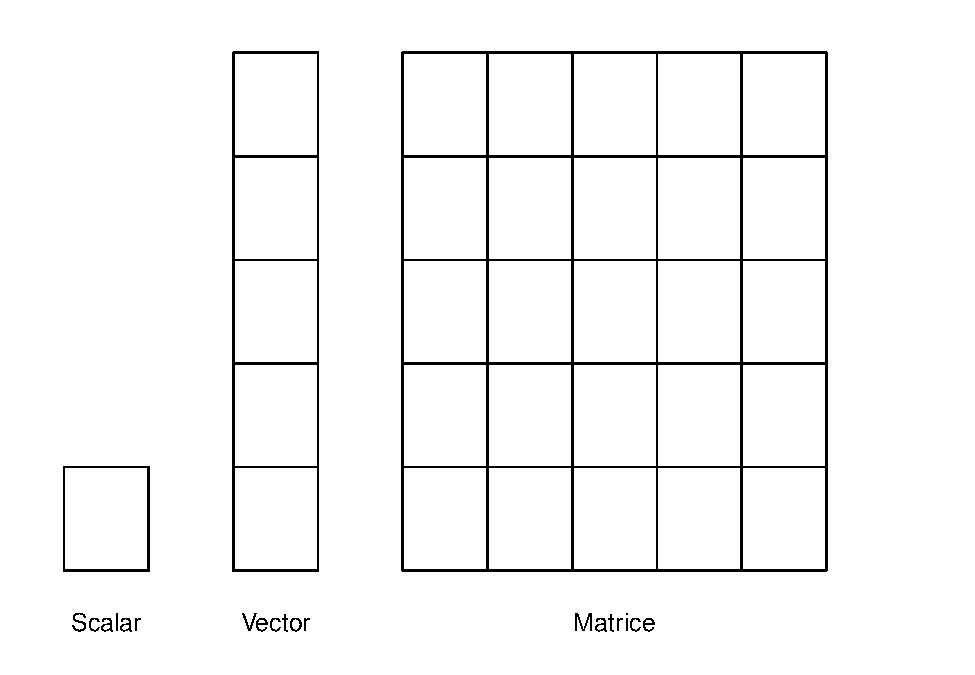
\includegraphics[width=0.8\linewidth]{Lab1_files/figure-latex/unnamed-chunk-30-1} 

}

\caption{Scalari, Vectori, Matrice}\label{fig:unnamed-chunk-30}
\end{figure}

Indexarea liniilor și a coloanelor pentru o matrice începe cu 1. De
exemplu, elementul din colțul din stânga sus al unei matrice este notat
cu \texttt{x{[}1,1{]}}. De asemenea este important de menționat că
stocarea (internă) a metricelor se face pe coloane în sensul că prima
oară este stocată coloana 1, apoi coloana 2, etc..

Există mai multe moduri de creare a unei matrici în R. Funcțiile cele
mai uzuale sunt prezentate în tabelul de mai jos. Cum matricele sunt
combinații de vectori, fiecare funcție primește ca argument unul sau mai
mulți vectori (toți de același tip) și ne întoarce o matrice.

\begin{longtable}[]{@{}lll@{}}
\caption{Functii care permit crearea matricelor}\tabularnewline
\toprule
\begin{minipage}[b]{0.20\columnwidth}\raggedright
Funcție\strut
\end{minipage} & \begin{minipage}[b]{0.28\columnwidth}\raggedright
Descriere\strut
\end{minipage} & \begin{minipage}[b]{0.44\columnwidth}\raggedright
Exemple\strut
\end{minipage}\tabularnewline
\midrule
\endfirsthead
\toprule
\begin{minipage}[b]{0.20\columnwidth}\raggedright
Funcție\strut
\end{minipage} & \begin{minipage}[b]{0.28\columnwidth}\raggedright
Descriere\strut
\end{minipage} & \begin{minipage}[b]{0.44\columnwidth}\raggedright
Exemple\strut
\end{minipage}\tabularnewline
\midrule
\endhead
\begin{minipage}[t]{0.20\columnwidth}\raggedright
\texttt{cbind(a,\ b,\ c)}\strut
\end{minipage} & \begin{minipage}[t]{0.28\columnwidth}\raggedright
Combină vectorii ca și coloane într-o matrice\strut
\end{minipage} & \begin{minipage}[t]{0.44\columnwidth}\raggedright
\texttt{cbind(1:5,\ 6:10,\ 11:15)}\strut
\end{minipage}\tabularnewline
\begin{minipage}[t]{0.20\columnwidth}\raggedright
\texttt{rbind(a,\ b,\ c)}\strut
\end{minipage} & \begin{minipage}[t]{0.28\columnwidth}\raggedright
Combină vectorii ca și linii într-o matrice\strut
\end{minipage} & \begin{minipage}[t]{0.44\columnwidth}\raggedright
\texttt{rbind(1:5,\ 6:10,\ 11:15)}\strut
\end{minipage}\tabularnewline
\begin{minipage}[t]{0.20\columnwidth}\raggedright
\texttt{matrix(x,\ nrow,\ ncol,\ byrow)}\strut
\end{minipage} & \begin{minipage}[t]{0.28\columnwidth}\raggedright
Crează o matrice dintr-un vector \texttt{x}\strut
\end{minipage} & \begin{minipage}[t]{0.44\columnwidth}\raggedright
\texttt{matrix(x\ =\ 1:12,\ nrow\ =\ 3,\ ncol\ =\ 4)}\strut
\end{minipage}\tabularnewline
\bottomrule
\end{longtable}

Pentru a vedea ce obținem atunci când folosim funcțiile \texttt{cbind()}
și \texttt{rbind()} să considerăm exemplele următoare:

\newpage

\begin{Shaded}
\begin{Highlighting}[]
\NormalTok{x <-}\StringTok{ }\DecValTok{1}\OperatorTok{:}\DecValTok{5}
\NormalTok{y <-}\StringTok{ }\DecValTok{6}\OperatorTok{:}\DecValTok{10}
\NormalTok{z <-}\StringTok{ }\DecValTok{11}\OperatorTok{:}\DecValTok{15}

\CommentTok{# Cream o matrice cu x, y si z ca si coloane}
\KeywordTok{cbind}\NormalTok{(x, y, z)}
\NormalTok{     x  y  z}
\NormalTok{[}\DecValTok{1}\NormalTok{,] }\DecValTok{1}  \DecValTok{6} \DecValTok{11}
\NormalTok{[}\DecValTok{2}\NormalTok{,] }\DecValTok{2}  \DecValTok{7} \DecValTok{12}
\NormalTok{[}\DecValTok{3}\NormalTok{,] }\DecValTok{3}  \DecValTok{8} \DecValTok{13}
\NormalTok{[}\DecValTok{4}\NormalTok{,] }\DecValTok{4}  \DecValTok{9} \DecValTok{14}
\NormalTok{[}\DecValTok{5}\NormalTok{,] }\DecValTok{5} \DecValTok{10} \DecValTok{15}

\CommentTok{# Cream o matrice in care x, y si z sunt linii}
\KeywordTok{rbind}\NormalTok{(x, y, z)}
\NormalTok{  [,}\DecValTok{1}\NormalTok{] [,}\DecValTok{2}\NormalTok{] [,}\DecValTok{3}\NormalTok{] [,}\DecValTok{4}\NormalTok{] [,}\DecValTok{5}\NormalTok{]}
\NormalTok{x    }\DecValTok{1}    \DecValTok{2}    \DecValTok{3}    \DecValTok{4}    \DecValTok{5}
\NormalTok{y    }\DecValTok{6}    \DecValTok{7}    \DecValTok{8}    \DecValTok{9}   \DecValTok{10}
\NormalTok{z   }\DecValTok{11}   \DecValTok{12}   \DecValTok{13}   \DecValTok{14}   \DecValTok{15}
\end{Highlighting}
\end{Shaded}

Funcția \texttt{matrix()} crează o matrice plecând de la un singur
vector. Funcția are patru valori de intrare: \texttt{data} -- un vector
cu date, \texttt{nrow} -- numărul de linii pe care le vrem în matrice,
\texttt{ncol} -- numărul de coloane pe care să le aibe matricea și
\texttt{byrow} -- o valoare logică care permite crearea matricei pe
linii (nu pe coloane cum este default-ul).

\begin{Shaded}
\begin{Highlighting}[]
\CommentTok{# matrice cu 5 linii si 2 coloane}
\KeywordTok{matrix}\NormalTok{(}\DataTypeTok{data =} \DecValTok{1}\OperatorTok{:}\DecValTok{10}\NormalTok{,}
       \DataTypeTok{nrow =} \DecValTok{5}\NormalTok{,}
       \DataTypeTok{ncol =} \DecValTok{2}\NormalTok{)}
\NormalTok{     [,}\DecValTok{1}\NormalTok{] [,}\DecValTok{2}\NormalTok{]}
\NormalTok{[}\DecValTok{1}\NormalTok{,]    }\DecValTok{1}    \DecValTok{6}
\NormalTok{[}\DecValTok{2}\NormalTok{,]    }\DecValTok{2}    \DecValTok{7}
\NormalTok{[}\DecValTok{3}\NormalTok{,]    }\DecValTok{3}    \DecValTok{8}
\NormalTok{[}\DecValTok{4}\NormalTok{,]    }\DecValTok{4}    \DecValTok{9}
\NormalTok{[}\DecValTok{5}\NormalTok{,]    }\DecValTok{5}   \DecValTok{10}

\CommentTok{# matrice cu 2 linii si 5 coloane}
\KeywordTok{matrix}\NormalTok{(}\DataTypeTok{data =} \DecValTok{1}\OperatorTok{:}\DecValTok{10}\NormalTok{,}
       \DataTypeTok{nrow =} \DecValTok{2}\NormalTok{,}
       \DataTypeTok{ncol =} \DecValTok{5}\NormalTok{)}
\NormalTok{     [,}\DecValTok{1}\NormalTok{] [,}\DecValTok{2}\NormalTok{] [,}\DecValTok{3}\NormalTok{] [,}\DecValTok{4}\NormalTok{] [,}\DecValTok{5}\NormalTok{]}
\NormalTok{[}\DecValTok{1}\NormalTok{,]    }\DecValTok{1}    \DecValTok{3}    \DecValTok{5}    \DecValTok{7}    \DecValTok{9}
\NormalTok{[}\DecValTok{2}\NormalTok{,]    }\DecValTok{2}    \DecValTok{4}    \DecValTok{6}    \DecValTok{8}   \DecValTok{10}

\CommentTok{# aceeasi matrice cu 2 linii si 5 coloane, umpluta pe linii }
\KeywordTok{matrix}\NormalTok{(}\DataTypeTok{data =} \DecValTok{1}\OperatorTok{:}\DecValTok{10}\NormalTok{,}
       \DataTypeTok{nrow =} \DecValTok{2}\NormalTok{,}
       \DataTypeTok{ncol =} \DecValTok{5}\NormalTok{,}
       \DataTypeTok{byrow =} \OtherTok{TRUE}\NormalTok{)}
\NormalTok{     [,}\DecValTok{1}\NormalTok{] [,}\DecValTok{2}\NormalTok{] [,}\DecValTok{3}\NormalTok{] [,}\DecValTok{4}\NormalTok{] [,}\DecValTok{5}\NormalTok{]}
\NormalTok{[}\DecValTok{1}\NormalTok{,]    }\DecValTok{1}    \DecValTok{2}    \DecValTok{3}    \DecValTok{4}    \DecValTok{5}
\NormalTok{[}\DecValTok{2}\NormalTok{,]    }\DecValTok{6}    \DecValTok{7}    \DecValTok{8}    \DecValTok{9}   \DecValTok{10}
\end{Highlighting}
\end{Shaded}

Operațiile uzuale cu vectori se aplică și matricelor. Pe lângă acestea
avem la dispoziție și operații de algebră liniară clasice, cum ar fi
determinarea dimensiunii acestora, transpunerea matricelor sau
înmulțirea lor:

\begin{Shaded}
\begin{Highlighting}[]
\KeywordTok{diag}\NormalTok{(M) }\CommentTok{# Diagonala matricei M}
\KeywordTok{dim}\NormalTok{(M) }\CommentTok{# Dimensiunile matricei M}
\KeywordTok{nrow}\NormalTok{(M) }\CommentTok{# Numarul de linii ale matricei M}
\KeywordTok{ncol}\NormalTok{(M) }\CommentTok{# Numarul de coloane ale matricei M}
\KeywordTok{t}\NormalTok{(M) }\CommentTok{# Transpusa}
\KeywordTok{colSums}\NormalTok{(M), }\KeywordTok{rowSums}\NormalTok{(M) }\CommentTok{# Suma pe coloane si suma pe linii}
\end{Highlighting}
\end{Shaded}

De exemplu:

\begin{Shaded}
\begin{Highlighting}[]
\NormalTok{m =}\StringTok{ }\KeywordTok{matrix}\NormalTok{(}\DataTypeTok{data =} \DecValTok{1}\OperatorTok{:}\DecValTok{10}\NormalTok{,}
       \DataTypeTok{nrow =} \DecValTok{2}\NormalTok{,}
       \DataTypeTok{ncol =} \DecValTok{5}\NormalTok{)}
\NormalTok{m}
\NormalTok{     [,}\DecValTok{1}\NormalTok{] [,}\DecValTok{2}\NormalTok{] [,}\DecValTok{3}\NormalTok{] [,}\DecValTok{4}\NormalTok{] [,}\DecValTok{5}\NormalTok{]}
\NormalTok{[}\DecValTok{1}\NormalTok{,]    }\DecValTok{1}    \DecValTok{3}    \DecValTok{5}    \DecValTok{7}    \DecValTok{9}
\NormalTok{[}\DecValTok{2}\NormalTok{,]    }\DecValTok{2}    \DecValTok{4}    \DecValTok{6}    \DecValTok{8}   \DecValTok{10}

\KeywordTok{dim}\NormalTok{(m) }\CommentTok{# dimensiunea matricei}
\NormalTok{[}\DecValTok{1}\NormalTok{] }\DecValTok{2} \DecValTok{5}
\KeywordTok{nrow}\NormalTok{(m) }\CommentTok{# numarul de linii}
\NormalTok{[}\DecValTok{1}\NormalTok{] }\DecValTok{2}
\KeywordTok{ncol}\NormalTok{(m) }\CommentTok{# numarul de coloane}
\NormalTok{[}\DecValTok{1}\NormalTok{] }\DecValTok{5}
\end{Highlighting}
\end{Shaded}

Adunarea și scăderea matricelor se face pe componenete:

\begin{Shaded}
\begin{Highlighting}[]
\NormalTok{A =}\StringTok{ }\KeywordTok{matrix}\NormalTok{(}\KeywordTok{c}\NormalTok{(}\DecValTok{1}\NormalTok{, }\DecValTok{3}\NormalTok{, }\DecValTok{2}\NormalTok{, }\DecValTok{2}\NormalTok{, }\DecValTok{2}\NormalTok{, }\DecValTok{1}\NormalTok{, }\DecValTok{3}\NormalTok{, }\DecValTok{1}\NormalTok{, }\DecValTok{3}\NormalTok{), }\DataTypeTok{ncol =} \DecValTok{3}\NormalTok{)}
\NormalTok{B =}\StringTok{ }\KeywordTok{matrix}\NormalTok{(}\KeywordTok{c}\NormalTok{(}\DecValTok{4}\NormalTok{, }\DecValTok{6}\NormalTok{, }\DecValTok{4}\NormalTok{, }\DecValTok{5}\NormalTok{, }\DecValTok{5}\NormalTok{, }\DecValTok{6}\NormalTok{, }\DecValTok{6}\NormalTok{, }\DecValTok{4}\NormalTok{, }\DecValTok{5}\NormalTok{), }\DataTypeTok{ncol =} \DecValTok{3}\NormalTok{)}
\NormalTok{a =}\StringTok{ }\DecValTok{2}

\NormalTok{A }\OperatorTok{+}\StringTok{ }\NormalTok{a}
\NormalTok{     [,}\DecValTok{1}\NormalTok{] [,}\DecValTok{2}\NormalTok{] [,}\DecValTok{3}\NormalTok{]}
\NormalTok{[}\DecValTok{1}\NormalTok{,]    }\DecValTok{3}    \DecValTok{4}    \DecValTok{5}
\NormalTok{[}\DecValTok{2}\NormalTok{,]    }\DecValTok{5}    \DecValTok{4}    \DecValTok{3}
\NormalTok{[}\DecValTok{3}\NormalTok{,]    }\DecValTok{4}    \DecValTok{3}    \DecValTok{5}
\NormalTok{A }\OperatorTok{+}\StringTok{ }\NormalTok{B}
\NormalTok{     [,}\DecValTok{1}\NormalTok{] [,}\DecValTok{2}\NormalTok{] [,}\DecValTok{3}\NormalTok{]}
\NormalTok{[}\DecValTok{1}\NormalTok{,]    }\DecValTok{5}    \DecValTok{7}    \DecValTok{9}
\NormalTok{[}\DecValTok{2}\NormalTok{,]    }\DecValTok{9}    \DecValTok{7}    \DecValTok{5}
\NormalTok{[}\DecValTok{3}\NormalTok{,]    }\DecValTok{6}    \DecValTok{7}    \DecValTok{8}
\NormalTok{A }\OperatorTok{-}\StringTok{ }\NormalTok{B}
\NormalTok{     [,}\DecValTok{1}\NormalTok{] [,}\DecValTok{2}\NormalTok{] [,}\DecValTok{3}\NormalTok{]}
\NormalTok{[}\DecValTok{1}\NormalTok{,]   }\DecValTok{-3}   \DecValTok{-3}   \DecValTok{-3}
\NormalTok{[}\DecValTok{2}\NormalTok{,]   }\DecValTok{-3}   \DecValTok{-3}   \DecValTok{-3}
\NormalTok{[}\DecValTok{3}\NormalTok{,]   }\DecValTok{-2}   \DecValTok{-5}   \DecValTok{-2}
\end{Highlighting}
\end{Shaded}

Înmulțirea și împărțirea se face tot pe componenete

\begin{Shaded}
\begin{Highlighting}[]
\NormalTok{A }\OperatorTok{*}\StringTok{ }\NormalTok{a}
\NormalTok{     [,}\DecValTok{1}\NormalTok{] [,}\DecValTok{2}\NormalTok{] [,}\DecValTok{3}\NormalTok{]}
\NormalTok{[}\DecValTok{1}\NormalTok{,]    }\DecValTok{2}    \DecValTok{4}    \DecValTok{6}
\NormalTok{[}\DecValTok{2}\NormalTok{,]    }\DecValTok{6}    \DecValTok{4}    \DecValTok{2}
\NormalTok{[}\DecValTok{3}\NormalTok{,]    }\DecValTok{4}    \DecValTok{2}    \DecValTok{6}
\NormalTok{A }\OperatorTok{*}\StringTok{ }\NormalTok{B}
\NormalTok{     [,}\DecValTok{1}\NormalTok{] [,}\DecValTok{2}\NormalTok{] [,}\DecValTok{3}\NormalTok{]}
\NormalTok{[}\DecValTok{1}\NormalTok{,]    }\DecValTok{4}   \DecValTok{10}   \DecValTok{18}
\NormalTok{[}\DecValTok{2}\NormalTok{,]   }\DecValTok{18}   \DecValTok{10}    \DecValTok{4}
\NormalTok{[}\DecValTok{3}\NormalTok{,]    }\DecValTok{8}    \DecValTok{6}   \DecValTok{15}
\NormalTok{A }\OperatorTok{/}\StringTok{ }\NormalTok{B}
\NormalTok{     [,}\DecValTok{1}\NormalTok{]      [,}\DecValTok{2}\NormalTok{] [,}\DecValTok{3}\NormalTok{]}
\NormalTok{[}\DecValTok{1}\NormalTok{,] }\FloatTok{0.25} \FloatTok{0.4000000} \FloatTok{0.50}
\NormalTok{[}\DecValTok{2}\NormalTok{,] }\FloatTok{0.50} \FloatTok{0.4000000} \FloatTok{0.25}
\NormalTok{[}\DecValTok{3}\NormalTok{,] }\FloatTok{0.50} \FloatTok{0.1666667} \FloatTok{0.60}
\end{Highlighting}
\end{Shaded}

Transpusa unei matrice (\(A^\intercal\)) se obține cu ajutorul funcției
\texttt{t()}

\begin{Shaded}
\begin{Highlighting}[]
\KeywordTok{t}\NormalTok{(A)}
\NormalTok{     [,}\DecValTok{1}\NormalTok{] [,}\DecValTok{2}\NormalTok{] [,}\DecValTok{3}\NormalTok{]}
\NormalTok{[}\DecValTok{1}\NormalTok{,]    }\DecValTok{1}    \DecValTok{3}    \DecValTok{2}
\NormalTok{[}\DecValTok{2}\NormalTok{,]    }\DecValTok{2}    \DecValTok{2}    \DecValTok{1}
\NormalTok{[}\DecValTok{3}\NormalTok{,]    }\DecValTok{3}    \DecValTok{1}    \DecValTok{3}
\end{Highlighting}
\end{Shaded}

iar inversa (\(A^{-1}\)) cu ajutorul funcției \texttt{solve()}

\begin{Shaded}
\begin{Highlighting}[]
\KeywordTok{solve}\NormalTok{(A)}
\NormalTok{            [,}\DecValTok{1}\NormalTok{]  [,}\DecValTok{2}\NormalTok{]       [,}\DecValTok{3}\NormalTok{]}
\NormalTok{[}\DecValTok{1}\NormalTok{,] }\FloatTok{-0.41666667}  \FloatTok{0.25}  \FloatTok{0.3333333}
\NormalTok{[}\DecValTok{2}\NormalTok{,]  }\FloatTok{0.58333333}  \FloatTok{0.25} \FloatTok{-0.6666667}
\NormalTok{[}\DecValTok{3}\NormalTok{,]  }\FloatTok{0.08333333} \FloatTok{-0.25}  \FloatTok{0.3333333}
\end{Highlighting}
\end{Shaded}

Înmulțirea (uzuală) a matricelor se face folosind operatorul
\texttt{\%*\%}

\begin{Shaded}
\begin{Highlighting}[]
\NormalTok{A }\OperatorTok\StringTok{ }\NormalTok{B }\CommentTok{# inmultirea matricelor}
\NormalTok{     [,}\DecValTok{1}\NormalTok{] [,}\DecValTok{2}\NormalTok{] [,}\DecValTok{3}\NormalTok{]}
\NormalTok{[}\DecValTok{1}\NormalTok{,]   }\DecValTok{28}   \DecValTok{33}   \DecValTok{29}
\NormalTok{[}\DecValTok{2}\NormalTok{,]   }\DecValTok{28}   \DecValTok{31}   \DecValTok{31}
\NormalTok{[}\DecValTok{3}\NormalTok{,]   }\DecValTok{26}   \DecValTok{33}   \DecValTok{31}
\end{Highlighting}
\end{Shaded}

iar funcția \texttt{crossprod()} calculează produsul \(A^\intercal B\)
(mai repede decât folosind instrucțiunea \texttt{t(A)\ \%*\%\ B})

\begin{Shaded}
\begin{Highlighting}[]
\KeywordTok{crossprod}\NormalTok{(A, B)}
\NormalTok{     [,}\DecValTok{1}\NormalTok{] [,}\DecValTok{2}\NormalTok{] [,}\DecValTok{3}\NormalTok{]}
\NormalTok{[}\DecValTok{1}\NormalTok{,]   }\DecValTok{30}   \DecValTok{32}   \DecValTok{28}
\NormalTok{[}\DecValTok{2}\NormalTok{,]   }\DecValTok{24}   \DecValTok{26}   \DecValTok{25}
\NormalTok{[}\DecValTok{3}\NormalTok{,]   }\DecValTok{30}   \DecValTok{38}   \DecValTok{37}
\end{Highlighting}
\end{Shaded}

Determinantul și urma unei matrice se obțin folosind funcțiile
\texttt{det()} și respectiv \texttt{sum(diag())}

\begin{Shaded}
\begin{Highlighting}[]
\KeywordTok{det}\NormalTok{(A) }\CommentTok{# determinantul}
\NormalTok{[}\DecValTok{1}\NormalTok{] }\DecValTok{-12}
\KeywordTok{sum}\NormalTok{(}\KeywordTok{diag}\NormalTok{(A)) }\CommentTok{# urma matricei A}
\NormalTok{[}\DecValTok{1}\NormalTok{] }\DecValTok{6}
\end{Highlighting}
\end{Shaded}

Metodele de indexare discutate pentru vectori se aplică și în cazul
matricelor (\texttt{{[},{]}}) numai că acum în loc să folosim un vector
să indexăm putem să folosim doi vectori. Sintaxa are structura generală
\texttt{m{[}linii,\ coloane{]}} unde \texttt{linii} și \texttt{coloane}
sunt vectori cu valori întregi.

\begin{Shaded}
\begin{Highlighting}[]
\NormalTok{m =}\StringTok{ }\KeywordTok{matrix}\NormalTok{(}\DecValTok{1}\OperatorTok{:}\DecValTok{20}\NormalTok{, }\DataTypeTok{nrow =} \DecValTok{4}\NormalTok{, }\DataTypeTok{byrow =} \OtherTok{TRUE}\NormalTok{)}

\CommentTok{# Linia 1}
\NormalTok{m[}\DecValTok{1}\NormalTok{, ]}
\NormalTok{[}\DecValTok{1}\NormalTok{] }\DecValTok{1} \DecValTok{2} \DecValTok{3} \DecValTok{4} \DecValTok{5}

\CommentTok{# Coloana 5}
\NormalTok{m[, }\DecValTok{5}\NormalTok{]}
\NormalTok{[}\DecValTok{1}\NormalTok{]  }\DecValTok{5} \DecValTok{10} \DecValTok{15} \DecValTok{20}

\CommentTok{# Liniile 2, 3 si coloanele 3, 4}
\NormalTok{m[}\DecValTok{2}\OperatorTok{:}\DecValTok{3}\NormalTok{, }\DecValTok{3}\OperatorTok{:}\DecValTok{4}\NormalTok{]}
\NormalTok{     [,}\DecValTok{1}\NormalTok{] [,}\DecValTok{2}\NormalTok{]}
\NormalTok{[}\DecValTok{1}\NormalTok{,]    }\DecValTok{8}    \DecValTok{9}
\NormalTok{[}\DecValTok{2}\NormalTok{,]   }\DecValTok{13}   \DecValTok{14}

\CommentTok{# Elementele din coloana 3 care corespund liniilor pentru care elementele }
\CommentTok{# de pe prima coloana sunt > 3}
\NormalTok{m[m[,}\DecValTok{1}\NormalTok{]}\OperatorTok{>}\DecValTok{3}\NormalTok{, }\DecValTok{3}\NormalTok{]}
\NormalTok{[}\DecValTok{1}\NormalTok{]  }\DecValTok{8} \DecValTok{13} \DecValTok{18}
\end{Highlighting}
\end{Shaded}

\hypertarget{liste}{%
\subsection{Liste}\label{liste}}

Spre deosebire de vectori în care toate elementele trebuie să aibă
același tip de dată, structura de dată din R de tip listă (\emph{list})
permite combinarea obiectelor de mai multe tipuri. Cu alte cuvinte, o
listă poate avea primul element un scalar, al doilea un vector, al
treilea o matrice iar cel de-al patrulea element poate fi o altă listă.
Tehnic listele sunt tot vectori, vectorii pe care i-am văzut anterior se
numesc \emph{vectori atomici}, deoarece elementele lor nu se pot diviza,
pe când listele se numesc \emph{vectori recursivi}.

Ca un prim exemplu să considerăm cazul unei baze de date de angajați.
Pentru fiecare angajat, ne dorim să stocăm numele angajatului (șir de
caractere), salariul (valoare numerică) și o valoare de tip logic care
poate reprezenta apartenența într-o asociație. Pentru crearea listei
folosim funcția \texttt{list()}:

\begin{Shaded}
\begin{Highlighting}[]
\NormalTok{a =}\StringTok{ }\KeywordTok{list}\NormalTok{(}\DataTypeTok{nume =} \StringTok{"Ionel"}\NormalTok{, }\DataTypeTok{salariu =} \DecValTok{1500}\NormalTok{, }\DataTypeTok{apartenenta =}\NormalTok{ T)}
\NormalTok{a}
\OperatorTok{$}\NormalTok{nume}
\NormalTok{[}\DecValTok{1}\NormalTok{] }\StringTok{"Ionel"}

\OperatorTok{$}\NormalTok{salariu}
\NormalTok{[}\DecValTok{1}\NormalTok{] }\DecValTok{1500}

\OperatorTok{$}\NormalTok{apartenenta}
\NormalTok{[}\DecValTok{1}\NormalTok{] }\OtherTok{TRUE}
\KeywordTok{str}\NormalTok{(a) }\CommentTok{# structura listei}
\NormalTok{List of }\DecValTok{3}
 \OperatorTok{$}\StringTok{ }\NormalTok{nume       }\OperatorTok{:}\StringTok{ }\NormalTok{chr }\StringTok{"Ionel"}
 \OperatorTok{$}\StringTok{ }\NormalTok{salariu    }\OperatorTok{:}\StringTok{ }\NormalTok{num }\DecValTok{1500}
 \OperatorTok{$}\StringTok{ }\NormalTok{apartenenta}\OperatorTok{:}\StringTok{ }\NormalTok{logi }\OtherTok{TRUE}
\KeywordTok{names}\NormalTok{(a) }\CommentTok{# numele listei}
\NormalTok{[}\DecValTok{1}\NormalTok{] }\StringTok{"nume"}        \StringTok{"salariu"}     \StringTok{"apartenenta"}
\end{Highlighting}
\end{Shaded}

Numele componentelor listei \texttt{a} (nume, salariu, apartenenta) nu
sunt obligatorii dar cu toate acestea pentru claritate sunt indicate:

\begin{Shaded}
\begin{Highlighting}[]
\NormalTok{a2 =}\StringTok{ }\KeywordTok{list}\NormalTok{(}\StringTok{"Ionel"}\NormalTok{, }\DecValTok{1500}\NormalTok{, T)}
\NormalTok{a2}
\NormalTok{[[}\DecValTok{1}\NormalTok{]]}
\NormalTok{[}\DecValTok{1}\NormalTok{] }\StringTok{"Ionel"}

\NormalTok{[[}\DecValTok{2}\NormalTok{]]}
\NormalTok{[}\DecValTok{1}\NormalTok{] }\DecValTok{1500}

\NormalTok{[[}\DecValTok{3}\NormalTok{]]}
\NormalTok{[}\DecValTok{1}\NormalTok{] }\OtherTok{TRUE}
\end{Highlighting}
\end{Shaded}

Deoarece listele sunt vectori ele pot fi create și prin intermediul
funcției \texttt{vector()}:

\begin{Shaded}
\begin{Highlighting}[]
\NormalTok{z <-}\StringTok{ }\KeywordTok{vector}\NormalTok{(}\DataTypeTok{mode=}\StringTok{"list"}\NormalTok{)}
\NormalTok{z}
\KeywordTok{list}\NormalTok{()}
\NormalTok{z[[}\StringTok{"a"}\NormalTok{]] =}\StringTok{ }\DecValTok{3}
\NormalTok{z}
\OperatorTok{$}\NormalTok{a}
\NormalTok{[}\DecValTok{1}\NormalTok{] }\DecValTok{3}
\end{Highlighting}
\end{Shaded}

\hypertarget{indexarea-listelor}{%
\subsubsection{Indexarea listelor}\label{indexarea-listelor}}

Elementele unei liste pot fi accesate în diferite moduri. Dacă dorim să
extragem primul element al listei atunci vom folosi indexarea care
folosește o singură pereche de paranteze pătrate \texttt{{[}{]}}

\begin{Shaded}
\begin{Highlighting}[]
\NormalTok{a[}\DecValTok{1}\NormalTok{]}
\OperatorTok{$}\NormalTok{nume}
\NormalTok{[}\DecValTok{1}\NormalTok{] }\StringTok{"Ionel"}
\NormalTok{a[}\DecValTok{2}\NormalTok{]}
\OperatorTok{$}\NormalTok{salariu}
\NormalTok{[}\DecValTok{1}\NormalTok{] }\DecValTok{1500}

\CommentTok{# ce obtinem cand extragem un element al listei a ?}
\KeywordTok{str}\NormalTok{(a[}\DecValTok{1}\NormalTok{]) }
\NormalTok{List of }\DecValTok{1}
 \OperatorTok{$}\StringTok{ }\NormalTok{nume}\OperatorTok{:}\StringTok{ }\NormalTok{chr }\StringTok{"Ionel"}
\end{Highlighting}
\end{Shaded}

În cazul în care vrem să accesăm structura de date corespunzătoare
elementului i al listei vom folosi două perechi de paranteze pătrate
\texttt{{[}{[}{]}{]}} sau în cazul în care lista are nume operatorul
\texttt{\$} urmat de numele elementului i.

\begin{Shaded}
\begin{Highlighting}[]
\NormalTok{a[[}\DecValTok{1}\NormalTok{]]}
\NormalTok{[}\DecValTok{1}\NormalTok{] }\StringTok{"Ionel"}
\NormalTok{a[[}\DecValTok{2}\NormalTok{]]}
\NormalTok{[}\DecValTok{1}\NormalTok{] }\DecValTok{1500}

\NormalTok{a}\OperatorTok{$}\NormalTok{nume}
\NormalTok{[}\DecValTok{1}\NormalTok{] }\StringTok{"Ionel"}
\NormalTok{a[[}\StringTok{"nume"}\NormalTok{]]}
\NormalTok{[}\DecValTok{1}\NormalTok{] }\StringTok{"Ionel"}
\end{Highlighting}
\end{Shaded}

Operațiile de adăugare, respectiv ștergere, a elementelor unei liste
sunt des întâlnite.

Putem adăuga elemente după ce o listă a fost creată folosind numele
componentei

\begin{Shaded}
\begin{Highlighting}[]
\NormalTok{z =}\StringTok{ }\KeywordTok{list}\NormalTok{(}\DataTypeTok{a =} \StringTok{"abc"}\NormalTok{, }\DataTypeTok{b =} \DecValTok{111}\NormalTok{, }\DataTypeTok{c =} \KeywordTok{c}\NormalTok{(}\OtherTok{TRUE}\NormalTok{, }\OtherTok{FALSE}\NormalTok{))}
\NormalTok{z}
\OperatorTok{$}\NormalTok{a}
\NormalTok{[}\DecValTok{1}\NormalTok{] }\StringTok{"abc"}

\OperatorTok{$}\NormalTok{b}
\NormalTok{[}\DecValTok{1}\NormalTok{] }\DecValTok{111}

\OperatorTok{$}\NormalTok{c}
\NormalTok{[}\DecValTok{1}\NormalTok{]  }\OtherTok{TRUE} \OtherTok{FALSE}
\NormalTok{z}\OperatorTok{$}\NormalTok{d =}\StringTok{ "un nou element"}
\NormalTok{z}
\OperatorTok{$}\NormalTok{a}
\NormalTok{[}\DecValTok{1}\NormalTok{] }\StringTok{"abc"}

\OperatorTok{$}\NormalTok{b}
\NormalTok{[}\DecValTok{1}\NormalTok{] }\DecValTok{111}

\OperatorTok{$}\NormalTok{c}
\NormalTok{[}\DecValTok{1}\NormalTok{]  }\OtherTok{TRUE} \OtherTok{FALSE}

\OperatorTok{$}\NormalTok{d}
\NormalTok{[}\DecValTok{1}\NormalTok{] }\StringTok{"un nou element"}
\end{Highlighting}
\end{Shaded}

sau indexare vectorială

\begin{Shaded}
\begin{Highlighting}[]
\NormalTok{z[[}\DecValTok{5}\NormalTok{]] =}\StringTok{ }\DecValTok{200}
\NormalTok{z[}\DecValTok{6}\OperatorTok{:}\DecValTok{7}\NormalTok{] =}\StringTok{ }\KeywordTok{c}\NormalTok{(}\StringTok{"unu"}\NormalTok{, }\StringTok{"doi"}\NormalTok{)}
\NormalTok{z}
\OperatorTok{$}\NormalTok{a}
\NormalTok{[}\DecValTok{1}\NormalTok{] }\StringTok{"abc"}

\OperatorTok{$}\NormalTok{b}
\NormalTok{[}\DecValTok{1}\NormalTok{] }\DecValTok{111}

\OperatorTok{$}\NormalTok{c}
\NormalTok{[}\DecValTok{1}\NormalTok{]  }\OtherTok{TRUE} \OtherTok{FALSE}

\OperatorTok{$}\NormalTok{d}
\NormalTok{[}\DecValTok{1}\NormalTok{] }\StringTok{"un nou element"}

\NormalTok{[[}\DecValTok{5}\NormalTok{]]}
\NormalTok{[}\DecValTok{1}\NormalTok{] }\DecValTok{200}

\NormalTok{[[}\DecValTok{6}\NormalTok{]]}
\NormalTok{[}\DecValTok{1}\NormalTok{] }\StringTok{"unu"}

\NormalTok{[[}\DecValTok{7}\NormalTok{]]}
\NormalTok{[}\DecValTok{1}\NormalTok{] }\StringTok{"doi"}
\end{Highlighting}
\end{Shaded}

Putem șterge o componentă a listei atribuindu-i valoarea \texttt{NULL}:

\begin{Shaded}
\begin{Highlighting}[]
\NormalTok{z[}\DecValTok{4}\NormalTok{] =}\StringTok{ }\OtherTok{NULL}
\NormalTok{z}
\OperatorTok{$}\NormalTok{a}
\NormalTok{[}\DecValTok{1}\NormalTok{] }\StringTok{"abc"}

\OperatorTok{$}\NormalTok{b}
\NormalTok{[}\DecValTok{1}\NormalTok{] }\DecValTok{111}

\OperatorTok{$}\NormalTok{c}
\NormalTok{[}\DecValTok{1}\NormalTok{]  }\OtherTok{TRUE} \OtherTok{FALSE}

\NormalTok{[[}\DecValTok{4}\NormalTok{]]}
\NormalTok{[}\DecValTok{1}\NormalTok{] }\DecValTok{200}

\NormalTok{[[}\DecValTok{5}\NormalTok{]]}
\NormalTok{[}\DecValTok{1}\NormalTok{] }\StringTok{"unu"}

\NormalTok{[[}\DecValTok{6}\NormalTok{]]}
\NormalTok{[}\DecValTok{1}\NormalTok{] }\StringTok{"doi"}
\end{Highlighting}
\end{Shaded}

Putem de asemenea să concatenăm două liste folosind funcția \texttt{c()}
și să determinăm lungimea noii liste cu funcția \texttt{length()}.

\begin{Shaded}
\begin{Highlighting}[]
\NormalTok{l1 =}\StringTok{ }\KeywordTok{list}\NormalTok{(}\DecValTok{1}\OperatorTok{:}\DecValTok{10}\NormalTok{, }\KeywordTok{matrix}\NormalTok{(}\DecValTok{1}\OperatorTok{:}\DecValTok{6}\NormalTok{, }\DataTypeTok{ncol =} \DecValTok{3}\NormalTok{), }\KeywordTok{c}\NormalTok{(T, F))}
\NormalTok{l2 =}\StringTok{ }\KeywordTok{list}\NormalTok{(}\KeywordTok{c}\NormalTok{(}\StringTok{"Ionel"}\NormalTok{, }\StringTok{"Maria"}\NormalTok{), }\KeywordTok{seq}\NormalTok{(}\DecValTok{1}\NormalTok{,}\DecValTok{10}\NormalTok{,}\DecValTok{2}\NormalTok{))}

\NormalTok{l3 =}\StringTok{ }\KeywordTok{c}\NormalTok{(l1, l2)}
\KeywordTok{length}\NormalTok{(l3)}
\NormalTok{[}\DecValTok{1}\NormalTok{] }\DecValTok{5}
\KeywordTok{str}\NormalTok{(l3)}
\NormalTok{List of }\DecValTok{5}
 \OperatorTok{$}\StringTok{ }\ErrorTok{:}\StringTok{ }\NormalTok{int [}\DecValTok{1}\OperatorTok{:}\DecValTok{10}\NormalTok{] }\DecValTok{1} \DecValTok{2} \DecValTok{3} \DecValTok{4} \DecValTok{5} \DecValTok{6} \DecValTok{7} \DecValTok{8} \DecValTok{9} \DecValTok{10}
 \OperatorTok{$}\StringTok{ }\ErrorTok{:}\StringTok{ }\NormalTok{int [}\DecValTok{1}\OperatorTok{:}\DecValTok{2}\NormalTok{, }\DecValTok{1}\OperatorTok{:}\DecValTok{3}\NormalTok{] }\DecValTok{1} \DecValTok{2} \DecValTok{3} \DecValTok{4} \DecValTok{5} \DecValTok{6}
 \OperatorTok{$}\StringTok{ }\ErrorTok{:}\StringTok{ }\NormalTok{logi [}\DecValTok{1}\OperatorTok{:}\DecValTok{2}\NormalTok{] }\OtherTok{TRUE} \OtherTok{FALSE}
 \OperatorTok{$}\StringTok{ }\ErrorTok{:}\StringTok{ }\NormalTok{chr [}\DecValTok{1}\OperatorTok{:}\DecValTok{2}\NormalTok{] }\StringTok{"Ionel"} \StringTok{"Maria"}
 \OperatorTok{$}\StringTok{ }\ErrorTok{:}\StringTok{ }\NormalTok{num [}\DecValTok{1}\OperatorTok{:}\DecValTok{5}\NormalTok{] }\DecValTok{1} \DecValTok{3} \DecValTok{5} \DecValTok{7} \DecValTok{9}
\end{Highlighting}
\end{Shaded}

\hypertarget{data-frame-uri}{%
\subsection{Data frame-uri}\label{data-frame-uri}}

La nivel intuitiv, o structură de date de tip \emph{data frame} este ca
o matrice, având o structură bidimensională cu linii și coloane. Cu
toate acestea ea diferă de structura de date de tip matrice prin faptul
că fiecare coloană poate avea tipuri de date diferite. Spre exemplu, o
coloană poate să conțină valori numerice pe când o alta, valori de tip
caracter sau logic. Din punct de vedere tehnic, o structură de tip data
frame este o listă a cărei componente sunt vectori (atomici) de lungimi
egale.

Pentru a crea un dataframe din vectori putem folosi funcția
\texttt{data.frame()}. Această funcție funcționează similar cu funcția
\texttt{list()} sau \texttt{cbind()}, diferența față de \texttt{cbind()}
este că avem posibilitatea să dăm nume coloanelor atunci când le unim.
Dată fiind flexibilitatea acestei structuri de date, majoritatea
seturilor de date din R sunt stocate sub formă de dataframe (această
structură de date este și cea mai des întâlnită în analiza statistică).

Să creăm un dataframe simplu numit \texttt{survey} folosind funcția
\texttt{data.frame()}:

\begin{Shaded}
\begin{Highlighting}[]
\NormalTok{survey <-}\StringTok{ }\KeywordTok{data.frame}\NormalTok{(}\StringTok{"index"}\NormalTok{ =}\StringTok{ }\KeywordTok{c}\NormalTok{(}\DecValTok{1}\NormalTok{, }\DecValTok{2}\NormalTok{, }\DecValTok{3}\NormalTok{, }\DecValTok{4}\NormalTok{, }\DecValTok{5}\NormalTok{),}
                     \StringTok{"sex"}\NormalTok{ =}\StringTok{ }\KeywordTok{c}\NormalTok{(}\StringTok{"m"}\NormalTok{, }\StringTok{"m"}\NormalTok{, }\StringTok{"m"}\NormalTok{, }\StringTok{"f"}\NormalTok{, }\StringTok{"f"}\NormalTok{),}
                     \StringTok{"age"}\NormalTok{ =}\StringTok{ }\KeywordTok{c}\NormalTok{(}\DecValTok{99}\NormalTok{, }\DecValTok{46}\NormalTok{, }\DecValTok{23}\NormalTok{, }\DecValTok{54}\NormalTok{, }\DecValTok{23}\NormalTok{))}
\NormalTok{survey}
\NormalTok{  index sex age}
\DecValTok{1}     \DecValTok{1}\NormalTok{   m  }\DecValTok{99}
\DecValTok{2}     \DecValTok{2}\NormalTok{   m  }\DecValTok{46}
\DecValTok{3}     \DecValTok{3}\NormalTok{   m  }\DecValTok{23}
\DecValTok{4}     \DecValTok{4}\NormalTok{   f  }\DecValTok{54}
\DecValTok{5}     \DecValTok{5}\NormalTok{   f  }\DecValTok{23}
\end{Highlighting}
\end{Shaded}

Funcția \texttt{data.frame()} prezintă un argument specific numit
\texttt{stringsAsFactors} care permite convertirea coloanelor ce conțin
elemente de tip caracter într-un tip de obiect numit \textbf{factor}. Un
factor este o variabilă nominală care poate lua un număr bine definit de
valori. De exemplu, putem crea o variabilă de tip factor \emph{sex} care
poate lua doar două valori: \emph{masculin} și \emph{feminin}.
Comportamentul implicit al funcției \texttt{data.frame()}
(\texttt{stringAsFactors\ =\ TRUE}) transformă automat coloanele de tip
caracter în factor, motiv pentru care trebuie să includem argumentul
\texttt{stringsAsFactors\ =\ FALSE}.

\begin{Shaded}
\begin{Highlighting}[]
\CommentTok{# Structura initiala}
\KeywordTok{str}\NormalTok{(survey)}
\StringTok{'data.frame'}\OperatorTok{:}\StringTok{   }\DecValTok{5}\NormalTok{ obs. of  }\DecValTok{3}\NormalTok{ variables}\OperatorTok{:}
\StringTok{ }\ErrorTok{$}\StringTok{ }\NormalTok{index}\OperatorTok{:}\StringTok{ }\NormalTok{num  }\DecValTok{1} \DecValTok{2} \DecValTok{3} \DecValTok{4} \DecValTok{5}
 \OperatorTok{$}\StringTok{ }\NormalTok{sex  }\OperatorTok{:}\StringTok{ }\NormalTok{Factor w}\OperatorTok{/}\StringTok{ }\DecValTok{2}\NormalTok{ levels }\StringTok{"f"}\NormalTok{,}\StringTok{"m"}\OperatorTok{:}\StringTok{ }\DecValTok{2} \DecValTok{2} \DecValTok{2} \DecValTok{1} \DecValTok{1}
 \OperatorTok{$}\StringTok{ }\NormalTok{age  }\OperatorTok{:}\StringTok{ }\NormalTok{num  }\DecValTok{99} \DecValTok{46} \DecValTok{23} \DecValTok{54} \DecValTok{23}

\NormalTok{survey <-}\StringTok{ }\KeywordTok{data.frame}\NormalTok{(}\StringTok{"index"}\NormalTok{ =}\StringTok{ }\KeywordTok{c}\NormalTok{(}\DecValTok{1}\NormalTok{, }\DecValTok{2}\NormalTok{, }\DecValTok{3}\NormalTok{, }\DecValTok{4}\NormalTok{, }\DecValTok{5}\NormalTok{),}
                     \StringTok{"sex"}\NormalTok{ =}\StringTok{ }\KeywordTok{c}\NormalTok{(}\StringTok{"m"}\NormalTok{, }\StringTok{"m"}\NormalTok{, }\StringTok{"m"}\NormalTok{, }\StringTok{"f"}\NormalTok{, }\StringTok{"f"}\NormalTok{),}
                     \StringTok{"age"}\NormalTok{ =}\StringTok{ }\KeywordTok{c}\NormalTok{(}\DecValTok{99}\NormalTok{, }\DecValTok{46}\NormalTok{, }\DecValTok{23}\NormalTok{, }\DecValTok{54}\NormalTok{, }\DecValTok{23}\NormalTok{),}
                     \DataTypeTok{stringsAsFactors =} \OtherTok{FALSE}\NormalTok{)}

\CommentTok{# Structura de dupa }
\KeywordTok{str}\NormalTok{(survey)}
\StringTok{'data.frame'}\OperatorTok{:}\StringTok{   }\DecValTok{5}\NormalTok{ obs. of  }\DecValTok{3}\NormalTok{ variables}\OperatorTok{:}
\StringTok{ }\ErrorTok{$}\StringTok{ }\NormalTok{index}\OperatorTok{:}\StringTok{ }\NormalTok{num  }\DecValTok{1} \DecValTok{2} \DecValTok{3} \DecValTok{4} \DecValTok{5}
 \OperatorTok{$}\StringTok{ }\NormalTok{sex  }\OperatorTok{:}\StringTok{ }\NormalTok{chr  }\StringTok{"m"} \StringTok{"m"} \StringTok{"m"} \StringTok{"f"}\NormalTok{ ...}
 \OperatorTok{$}\StringTok{ }\NormalTok{age  }\OperatorTok{:}\StringTok{ }\NormalTok{num  }\DecValTok{99} \DecValTok{46} \DecValTok{23} \DecValTok{54} \DecValTok{23}
\end{Highlighting}
\end{Shaded}

R are mai multe funcții care permit vizualizarea structurilor de tip
dataframe. Tabelul de mai jos include câteva astfel de funcții:

\begin{longtable}[]{@{}ll@{}}
\caption{Exemple de functii necesare pentru intelegerea structurii
dataframe-ului}\tabularnewline
\toprule
Funcție & Descriere\tabularnewline
\midrule
\endfirsthead
\toprule
Funcție & Descriere\tabularnewline
\midrule
\endhead
\texttt{head(x),\ tail(x)} & Printarea primelor linii (sau ultimelor
linii).\tabularnewline
\texttt{View(x)} & Vizualizarea obiectului într-o fereastră nouă,
tabelară.\tabularnewline
\texttt{nrow(x),\ ncol(x),\ dim(x)} & Numărul de linii și de
coloane.\tabularnewline
\texttt{rownames(),\ colnames(),\ names()} & Numele liniilor sau
coloanelor.\tabularnewline
\texttt{str(x)} & Structura dataframe-ului\tabularnewline
\bottomrule
\end{longtable}

\begin{Shaded}
\begin{Highlighting}[]
\KeywordTok{data}\NormalTok{() }\CommentTok{# vedem ce seturi de date exista}
\end{Highlighting}
\end{Shaded}

\begin{Shaded}
\begin{Highlighting}[]
\CommentTok{# Alegem setul de date mtcars}
\NormalTok{?mtcars}
\KeywordTok{str}\NormalTok{(mtcars) }\CommentTok{# structura setului de date}
\StringTok{'data.frame'}\OperatorTok{:}\StringTok{   }\DecValTok{32}\NormalTok{ obs. of  }\DecValTok{11}\NormalTok{ variables}\OperatorTok{:}
\StringTok{ }\ErrorTok{$}\StringTok{ }\NormalTok{mpg }\OperatorTok{:}\StringTok{ }\NormalTok{num  }\DecValTok{21} \DecValTok{21} \FloatTok{22.8} \FloatTok{21.4} \FloatTok{18.7} \FloatTok{18.1} \FloatTok{14.3} \FloatTok{24.4} \FloatTok{22.8} \FloatTok{19.2}\NormalTok{ ...}
 \OperatorTok{$}\StringTok{ }\NormalTok{cyl }\OperatorTok{:}\StringTok{ }\NormalTok{num  }\DecValTok{6} \DecValTok{6} \DecValTok{4} \DecValTok{6} \DecValTok{8} \DecValTok{6} \DecValTok{8} \DecValTok{4} \DecValTok{4} \DecValTok{6}\NormalTok{ ...}
 \OperatorTok{$}\StringTok{ }\NormalTok{disp}\OperatorTok{:}\StringTok{ }\NormalTok{num  }\DecValTok{160} \DecValTok{160} \DecValTok{108} \DecValTok{258} \DecValTok{360}\NormalTok{ ...}
 \OperatorTok{$}\StringTok{ }\NormalTok{hp  }\OperatorTok{:}\StringTok{ }\NormalTok{num  }\DecValTok{110} \DecValTok{110} \DecValTok{93} \DecValTok{110} \DecValTok{175} \DecValTok{105} \DecValTok{245} \DecValTok{62} \DecValTok{95} \DecValTok{123}\NormalTok{ ...}
 \OperatorTok{$}\StringTok{ }\NormalTok{drat}\OperatorTok{:}\StringTok{ }\NormalTok{num  }\FloatTok{3.9} \FloatTok{3.9} \FloatTok{3.85} \FloatTok{3.08} \FloatTok{3.15} \FloatTok{2.76} \FloatTok{3.21} \FloatTok{3.69} \FloatTok{3.92} \FloatTok{3.92}\NormalTok{ ...}
 \OperatorTok{$}\StringTok{ }\NormalTok{wt  }\OperatorTok{:}\StringTok{ }\NormalTok{num  }\FloatTok{2.62} \FloatTok{2.88} \FloatTok{2.32} \FloatTok{3.21} \FloatTok{3.44}\NormalTok{ ...}
 \OperatorTok{$}\StringTok{ }\NormalTok{qsec}\OperatorTok{:}\StringTok{ }\NormalTok{num  }\FloatTok{16.5} \DecValTok{17} \FloatTok{18.6} \FloatTok{19.4} \DecValTok{17}\NormalTok{ ...}
 \OperatorTok{$}\StringTok{ }\NormalTok{vs  }\OperatorTok{:}\StringTok{ }\NormalTok{num  }\DecValTok{0} \DecValTok{0} \DecValTok{1} \DecValTok{1} \DecValTok{0} \DecValTok{1} \DecValTok{0} \DecValTok{1} \DecValTok{1} \DecValTok{1}\NormalTok{ ...}
 \OperatorTok{$}\StringTok{ }\NormalTok{am  }\OperatorTok{:}\StringTok{ }\NormalTok{num  }\DecValTok{1} \DecValTok{1} \DecValTok{1} \DecValTok{0} \DecValTok{0} \DecValTok{0} \DecValTok{0} \DecValTok{0} \DecValTok{0} \DecValTok{0}\NormalTok{ ...}
 \OperatorTok{$}\StringTok{ }\NormalTok{gear}\OperatorTok{:}\StringTok{ }\NormalTok{num  }\DecValTok{4} \DecValTok{4} \DecValTok{4} \DecValTok{3} \DecValTok{3} \DecValTok{3} \DecValTok{3} \DecValTok{4} \DecValTok{4} \DecValTok{4}\NormalTok{ ...}
 \OperatorTok{$}\StringTok{ }\NormalTok{carb}\OperatorTok{:}\StringTok{ }\NormalTok{num  }\DecValTok{4} \DecValTok{4} \DecValTok{1} \DecValTok{1} \DecValTok{2} \DecValTok{1} \DecValTok{4} \DecValTok{2} \DecValTok{2} \DecValTok{4}\NormalTok{ ...}
\KeywordTok{head}\NormalTok{(mtcars)}
\NormalTok{                   mpg cyl disp  hp drat    wt  qsec vs am gear carb}
\NormalTok{Mazda RX4         }\FloatTok{21.0}   \DecValTok{6}  \DecValTok{160} \DecValTok{110} \FloatTok{3.90} \FloatTok{2.620} \FloatTok{16.46}  \DecValTok{0}  \DecValTok{1}    \DecValTok{4}    \DecValTok{4}
\NormalTok{Mazda RX4 Wag     }\FloatTok{21.0}   \DecValTok{6}  \DecValTok{160} \DecValTok{110} \FloatTok{3.90} \FloatTok{2.875} \FloatTok{17.02}  \DecValTok{0}  \DecValTok{1}    \DecValTok{4}    \DecValTok{4}
\NormalTok{Datsun }\DecValTok{710}        \FloatTok{22.8}   \DecValTok{4}  \DecValTok{108}  \DecValTok{93} \FloatTok{3.85} \FloatTok{2.320} \FloatTok{18.61}  \DecValTok{1}  \DecValTok{1}    \DecValTok{4}    \DecValTok{1}
\NormalTok{Hornet }\DecValTok{4}\NormalTok{ Drive    }\FloatTok{21.4}   \DecValTok{6}  \DecValTok{258} \DecValTok{110} \FloatTok{3.08} \FloatTok{3.215} \FloatTok{19.44}  \DecValTok{1}  \DecValTok{0}    \DecValTok{3}    \DecValTok{1}
\NormalTok{Hornet Sportabout }\FloatTok{18.7}   \DecValTok{8}  \DecValTok{360} \DecValTok{175} \FloatTok{3.15} \FloatTok{3.440} \FloatTok{17.02}  \DecValTok{0}  \DecValTok{0}    \DecValTok{3}    \DecValTok{2}
\NormalTok{Valiant           }\FloatTok{18.1}   \DecValTok{6}  \DecValTok{225} \DecValTok{105} \FloatTok{2.76} \FloatTok{3.460} \FloatTok{20.22}  \DecValTok{1}  \DecValTok{0}    \DecValTok{3}    \DecValTok{1}
\KeywordTok{tail}\NormalTok{(mtcars)}
\NormalTok{                mpg cyl  disp  hp drat    wt qsec vs am gear carb}
\NormalTok{Porsche }\DecValTok{914-2}  \FloatTok{26.0}   \DecValTok{4} \FloatTok{120.3}  \DecValTok{91} \FloatTok{4.43} \FloatTok{2.140} \FloatTok{16.7}  \DecValTok{0}  \DecValTok{1}    \DecValTok{5}    \DecValTok{2}
\NormalTok{Lotus Europa   }\FloatTok{30.4}   \DecValTok{4}  \FloatTok{95.1} \DecValTok{113} \FloatTok{3.77} \FloatTok{1.513} \FloatTok{16.9}  \DecValTok{1}  \DecValTok{1}    \DecValTok{5}    \DecValTok{2}
\NormalTok{Ford Pantera L }\FloatTok{15.8}   \DecValTok{8} \FloatTok{351.0} \DecValTok{264} \FloatTok{4.22} \FloatTok{3.170} \FloatTok{14.5}  \DecValTok{0}  \DecValTok{1}    \DecValTok{5}    \DecValTok{4}
\NormalTok{Ferrari Dino   }\FloatTok{19.7}   \DecValTok{6} \FloatTok{145.0} \DecValTok{175} \FloatTok{3.62} \FloatTok{2.770} \FloatTok{15.5}  \DecValTok{0}  \DecValTok{1}    \DecValTok{5}    \DecValTok{6}
\NormalTok{Maserati Bora  }\FloatTok{15.0}   \DecValTok{8} \FloatTok{301.0} \DecValTok{335} \FloatTok{3.54} \FloatTok{3.570} \FloatTok{14.6}  \DecValTok{0}  \DecValTok{1}    \DecValTok{5}    \DecValTok{8}
\NormalTok{Volvo 142E     }\FloatTok{21.4}   \DecValTok{4} \FloatTok{121.0} \DecValTok{109} \FloatTok{4.11} \FloatTok{2.780} \FloatTok{18.6}  \DecValTok{1}  \DecValTok{1}    \DecValTok{4}    \DecValTok{2}

\KeywordTok{rownames}\NormalTok{(mtcars)}
\NormalTok{ [}\DecValTok{1}\NormalTok{] }\StringTok{"Mazda RX4"}           \StringTok{"Mazda RX4 Wag"}       \StringTok{"Datsun 710"}         
\NormalTok{ [}\DecValTok{4}\NormalTok{] }\StringTok{"Hornet 4 Drive"}      \StringTok{"Hornet Sportabout"}   \StringTok{"Valiant"}            
\NormalTok{ [}\DecValTok{7}\NormalTok{] }\StringTok{"Duster 360"}          \StringTok{"Merc 240D"}           \StringTok{"Merc 230"}           
\NormalTok{[}\DecValTok{10}\NormalTok{] }\StringTok{"Merc 280"}            \StringTok{"Merc 280C"}           \StringTok{"Merc 450SE"}         
\NormalTok{[}\DecValTok{13}\NormalTok{] }\StringTok{"Merc 450SL"}          \StringTok{"Merc 450SLC"}         \StringTok{"Cadillac Fleetwood"} 
\NormalTok{[}\DecValTok{16}\NormalTok{] }\StringTok{"Lincoln Continental"} \StringTok{"Chrysler Imperial"}   \StringTok{"Fiat 128"}           
\NormalTok{[}\DecValTok{19}\NormalTok{] }\StringTok{"Honda Civic"}         \StringTok{"Toyota Corolla"}      \StringTok{"Toyota Corona"}      
\NormalTok{[}\DecValTok{22}\NormalTok{] }\StringTok{"Dodge Challenger"}    \StringTok{"AMC Javelin"}         \StringTok{"Camaro Z28"}         
\NormalTok{[}\DecValTok{25}\NormalTok{] }\StringTok{"Pontiac Firebird"}    \StringTok{"Fiat X1-9"}           \StringTok{"Porsche 914-2"}      
\NormalTok{[}\DecValTok{28}\NormalTok{] }\StringTok{"Lotus Europa"}        \StringTok{"Ford Pantera L"}      \StringTok{"Ferrari Dino"}       
\NormalTok{[}\DecValTok{31}\NormalTok{] }\StringTok{"Maserati Bora"}       \StringTok{"Volvo 142E"}         
\KeywordTok{names}\NormalTok{(mtcars)}
\NormalTok{ [}\DecValTok{1}\NormalTok{] }\StringTok{"mpg"}  \StringTok{"cyl"}  \StringTok{"disp"} \StringTok{"hp"}   \StringTok{"drat"} \StringTok{"wt"}   \StringTok{"qsec"} \StringTok{"vs"}   \StringTok{"am"}   \StringTok{"gear"}
\NormalTok{[}\DecValTok{11}\NormalTok{] }\StringTok{"carb"}
\end{Highlighting}
\end{Shaded}

\begin{Shaded}
\begin{Highlighting}[]
\KeywordTok{View}\NormalTok{(mtcars) }
\end{Highlighting}
\end{Shaded}

\hypertarget{metode-de-indexare}{%
\subsubsection{Metode de indexare}\label{metode-de-indexare}}

Indexarea structurilor de tip dataframe se face la fel ca și indexarea
listelor.

\begin{Shaded}
\begin{Highlighting}[]
\NormalTok{mtcars[}\DecValTok{1}\NormalTok{,}\DecValTok{1}\OperatorTok{:}\DecValTok{4}\NormalTok{]}
\NormalTok{          mpg cyl disp  hp}
\NormalTok{Mazda RX4  }\DecValTok{21}   \DecValTok{6}  \DecValTok{160} \DecValTok{110}
\NormalTok{mtcars[}\KeywordTok{c}\NormalTok{(}\DecValTok{1}\NormalTok{,}\DecValTok{2}\NormalTok{),}\DecValTok{2}\NormalTok{]}
\NormalTok{[}\DecValTok{1}\NormalTok{] }\DecValTok{6} \DecValTok{6}
\NormalTok{mtcars}\OperatorTok{$}\NormalTok{mpg}
\NormalTok{ [}\DecValTok{1}\NormalTok{] }\FloatTok{21.0} \FloatTok{21.0} \FloatTok{22.8} \FloatTok{21.4} \FloatTok{18.7} \FloatTok{18.1} \FloatTok{14.3} \FloatTok{24.4} \FloatTok{22.8} \FloatTok{19.2} \FloatTok{17.8} \FloatTok{16.4} \FloatTok{17.3} \FloatTok{15.2}
\NormalTok{[}\DecValTok{15}\NormalTok{] }\FloatTok{10.4} \FloatTok{10.4} \FloatTok{14.7} \FloatTok{32.4} \FloatTok{30.4} \FloatTok{33.9} \FloatTok{21.5} \FloatTok{15.5} \FloatTok{15.2} \FloatTok{13.3} \FloatTok{19.2} \FloatTok{27.3} \FloatTok{26.0} \FloatTok{30.4}
\NormalTok{[}\DecValTok{29}\NormalTok{] }\FloatTok{15.8} \FloatTok{19.7} \FloatTok{15.0} \FloatTok{21.4}
\end{Highlighting}
\end{Shaded}

La fel ca vectorii, dataframe-urile (dar și listele) pot fi indexate
logic

\begin{Shaded}
\begin{Highlighting}[]
\NormalTok{mtcars[mtcars}\OperatorTok{$}\NormalTok{mpg }\OperatorTok{>}\StringTok{ }\DecValTok{25}\NormalTok{, ]}
\NormalTok{                mpg cyl  disp  hp drat    wt  qsec vs am gear carb}
\NormalTok{Fiat }\DecValTok{128}       \FloatTok{32.4}   \DecValTok{4}  \FloatTok{78.7}  \DecValTok{66} \FloatTok{4.08} \FloatTok{2.200} \FloatTok{19.47}  \DecValTok{1}  \DecValTok{1}    \DecValTok{4}    \DecValTok{1}
\NormalTok{Honda Civic    }\FloatTok{30.4}   \DecValTok{4}  \FloatTok{75.7}  \DecValTok{52} \FloatTok{4.93} \FloatTok{1.615} \FloatTok{18.52}  \DecValTok{1}  \DecValTok{1}    \DecValTok{4}    \DecValTok{2}
\NormalTok{Toyota Corolla }\FloatTok{33.9}   \DecValTok{4}  \FloatTok{71.1}  \DecValTok{65} \FloatTok{4.22} \FloatTok{1.835} \FloatTok{19.90}  \DecValTok{1}  \DecValTok{1}    \DecValTok{4}    \DecValTok{1}
\NormalTok{Fiat X1}\DecValTok{-9}      \FloatTok{27.3}   \DecValTok{4}  \FloatTok{79.0}  \DecValTok{66} \FloatTok{4.08} \FloatTok{1.935} \FloatTok{18.90}  \DecValTok{1}  \DecValTok{1}    \DecValTok{4}    \DecValTok{1}
\NormalTok{Porsche }\DecValTok{914-2}  \FloatTok{26.0}   \DecValTok{4} \FloatTok{120.3}  \DecValTok{91} \FloatTok{4.43} \FloatTok{2.140} \FloatTok{16.70}  \DecValTok{0}  \DecValTok{1}    \DecValTok{5}    \DecValTok{2}
\NormalTok{Lotus Europa   }\FloatTok{30.4}   \DecValTok{4}  \FloatTok{95.1} \DecValTok{113} \FloatTok{3.77} \FloatTok{1.513} \FloatTok{16.90}  \DecValTok{1}  \DecValTok{1}    \DecValTok{5}    \DecValTok{2}
\NormalTok{mtcars[(mtcars}\OperatorTok{$}\NormalTok{mpg }\OperatorTok{>}\StringTok{ }\DecValTok{25}\NormalTok{) }\OperatorTok{&}\StringTok{ }\NormalTok{(mtcars}\OperatorTok{$}\NormalTok{wt }\OperatorTok{<}\StringTok{ }\FloatTok{1.8}\NormalTok{), ]}
\NormalTok{              mpg cyl disp  hp drat    wt  qsec vs am gear carb}
\NormalTok{Honda Civic  }\FloatTok{30.4}   \DecValTok{4} \FloatTok{75.7}  \DecValTok{52} \FloatTok{4.93} \FloatTok{1.615} \FloatTok{18.52}  \DecValTok{1}  \DecValTok{1}    \DecValTok{4}    \DecValTok{2}
\NormalTok{Lotus Europa }\FloatTok{30.4}   \DecValTok{4} \FloatTok{95.1} \DecValTok{113} \FloatTok{3.77} \FloatTok{1.513} \FloatTok{16.90}  \DecValTok{1}  \DecValTok{1}    \DecValTok{5}    \DecValTok{2}
\end{Highlighting}
\end{Shaded}

O altă metodă de indexare este prin folosirea funcției
\texttt{subset()}.

\begin{longtable}[]{@{}ll@{}}
\caption{Principalele argumente ale functiei subset()}\tabularnewline
\toprule
Argument & Descriere\tabularnewline
\midrule
\endfirsthead
\toprule
Argument & Descriere\tabularnewline
\midrule
\endhead
\texttt{x} & Un dataframe\tabularnewline
\texttt{subset} & Un vector logic care indică liniile pe care le
vrem\tabularnewline
\texttt{select} & Coloanele pe care vrem să le păstrăm\tabularnewline
\bottomrule
\end{longtable}

\begin{Shaded}
\begin{Highlighting}[]
\KeywordTok{subset}\NormalTok{(}\DataTypeTok{x =}\NormalTok{ mtcars,}
      \DataTypeTok{subset =}\NormalTok{ mpg }\OperatorTok{<}\StringTok{ }\DecValTok{12} \OperatorTok{&}
\StringTok{               }\NormalTok{cyl }\OperatorTok{>}\StringTok{ }\DecValTok{6}\NormalTok{,}
      \DataTypeTok{select =} \KeywordTok{c}\NormalTok{(disp, wt))}
\NormalTok{                    disp    wt}
\NormalTok{Cadillac Fleetwood   }\DecValTok{472} \FloatTok{5.250}
\NormalTok{Lincoln Continental  }\DecValTok{460} \FloatTok{5.424}
\end{Highlighting}
\end{Shaded}

\hypertarget{metode-de-manipulare}{%
\subsubsection{Metode de manipulare}\label{metode-de-manipulare}}

În această secțiune vom prezenta câteva metode mai avansate de
manipulare a seturilor de date (a data frame-urilor).

Vom începe prin introducerea comenzii \texttt{order()} care permite
sortarea liniilor unui data.frame în funcție de valorile coloanei de
interes. De exemplu să considerăm cazul setului de date \texttt{mtcars}.
Vrem să afisăm primele 10 mașini în funcție de greutatea lor (crescător
și descrescător):

\begin{Shaded}
\begin{Highlighting}[]
\NormalTok{cars_increasing =}\StringTok{ }\KeywordTok{rownames}\NormalTok{(mtcars[}\KeywordTok{order}\NormalTok{(mtcars}\OperatorTok{$}\NormalTok{wt),])}
\CommentTok{# afisarea celor mai usoare 10 masini}
\NormalTok{cars_increasing[}\DecValTok{1}\OperatorTok{:}\DecValTok{10}\NormalTok{]}
\NormalTok{ [}\DecValTok{1}\NormalTok{] }\StringTok{"Lotus Europa"}   \StringTok{"Honda Civic"}    \StringTok{"Toyota Corolla"} \StringTok{"Fiat X1-9"}     
\NormalTok{ [}\DecValTok{5}\NormalTok{] }\StringTok{"Porsche 914-2"}  \StringTok{"Fiat 128"}       \StringTok{"Datsun 710"}     \StringTok{"Toyota Corona"} 
\NormalTok{ [}\DecValTok{9}\NormalTok{] }\StringTok{"Mazda RX4"}      \StringTok{"Ferrari Dino"}  

\NormalTok{cars_decreasing =}\StringTok{ }\KeywordTok{rownames}\NormalTok{(mtcars[}\KeywordTok{order}\NormalTok{(mtcars}\OperatorTok{$}\NormalTok{wt, }\DataTypeTok{decreasing =} \OtherTok{TRUE}\NormalTok{),])}
\CommentTok{# afisarea celor mai grele 10 masini}
\NormalTok{cars_decreasing[}\DecValTok{1}\OperatorTok{:}\DecValTok{10}\NormalTok{]}
\NormalTok{ [}\DecValTok{1}\NormalTok{] }\StringTok{"Lincoln Continental"} \StringTok{"Chrysler Imperial"}   \StringTok{"Cadillac Fleetwood"} 
\NormalTok{ [}\DecValTok{4}\NormalTok{] }\StringTok{"Merc 450SE"}          \StringTok{"Pontiac Firebird"}    \StringTok{"Camaro Z28"}         
\NormalTok{ [}\DecValTok{7}\NormalTok{] }\StringTok{"Merc 450SLC"}         \StringTok{"Merc 450SL"}          \StringTok{"Duster 360"}         
\NormalTok{[}\DecValTok{10}\NormalTok{] }\StringTok{"Maserati Bora"}      
\end{Highlighting}
\end{Shaded}

Funcția \texttt{order()} permite ordonarea după mai mult de o coloană,
de exemplu dacă vrem să ordonăm mașinile după numărul de cilindrii și
după greutate atunci apelăm

\begin{Shaded}
\begin{Highlighting}[]
\NormalTok{mtcars[}\KeywordTok{order}\NormalTok{(mtcars}\OperatorTok{$}\NormalTok{cyl, mtcars}\OperatorTok{$}\NormalTok{wt), }\DecValTok{1}\OperatorTok{:}\DecValTok{6}\NormalTok{]}
\NormalTok{                     mpg cyl  disp  hp drat    wt}
\NormalTok{Lotus Europa        }\FloatTok{30.4}   \DecValTok{4}  \FloatTok{95.1} \DecValTok{113} \FloatTok{3.77} \FloatTok{1.513}
\NormalTok{Honda Civic         }\FloatTok{30.4}   \DecValTok{4}  \FloatTok{75.7}  \DecValTok{52} \FloatTok{4.93} \FloatTok{1.615}
\NormalTok{Toyota Corolla      }\FloatTok{33.9}   \DecValTok{4}  \FloatTok{71.1}  \DecValTok{65} \FloatTok{4.22} \FloatTok{1.835}
\NormalTok{Fiat X1}\DecValTok{-9}           \FloatTok{27.3}   \DecValTok{4}  \FloatTok{79.0}  \DecValTok{66} \FloatTok{4.08} \FloatTok{1.935}
\NormalTok{Porsche }\DecValTok{914-2}       \FloatTok{26.0}   \DecValTok{4} \FloatTok{120.3}  \DecValTok{91} \FloatTok{4.43} \FloatTok{2.140}
\NormalTok{Fiat }\DecValTok{128}            \FloatTok{32.4}   \DecValTok{4}  \FloatTok{78.7}  \DecValTok{66} \FloatTok{4.08} \FloatTok{2.200}
\NormalTok{Datsun }\DecValTok{710}          \FloatTok{22.8}   \DecValTok{4} \FloatTok{108.0}  \DecValTok{93} \FloatTok{3.85} \FloatTok{2.320}
\NormalTok{Toyota Corona       }\FloatTok{21.5}   \DecValTok{4} \FloatTok{120.1}  \DecValTok{97} \FloatTok{3.70} \FloatTok{2.465}
\NormalTok{Volvo 142E          }\FloatTok{21.4}   \DecValTok{4} \FloatTok{121.0} \DecValTok{109} \FloatTok{4.11} \FloatTok{2.780}
\NormalTok{Merc }\DecValTok{230}            \FloatTok{22.8}   \DecValTok{4} \FloatTok{140.8}  \DecValTok{95} \FloatTok{3.92} \FloatTok{3.150}
\NormalTok{Merc 240D           }\FloatTok{24.4}   \DecValTok{4} \FloatTok{146.7}  \DecValTok{62} \FloatTok{3.69} \FloatTok{3.190}
\NormalTok{Mazda RX4           }\FloatTok{21.0}   \DecValTok{6} \FloatTok{160.0} \DecValTok{110} \FloatTok{3.90} \FloatTok{2.620}
\NormalTok{Ferrari Dino        }\FloatTok{19.7}   \DecValTok{6} \FloatTok{145.0} \DecValTok{175} \FloatTok{3.62} \FloatTok{2.770}
\NormalTok{Mazda RX4 Wag       }\FloatTok{21.0}   \DecValTok{6} \FloatTok{160.0} \DecValTok{110} \FloatTok{3.90} \FloatTok{2.875}
\NormalTok{Hornet }\DecValTok{4}\NormalTok{ Drive      }\FloatTok{21.4}   \DecValTok{6} \FloatTok{258.0} \DecValTok{110} \FloatTok{3.08} \FloatTok{3.215}
\NormalTok{Merc }\DecValTok{280}            \FloatTok{19.2}   \DecValTok{6} \FloatTok{167.6} \DecValTok{123} \FloatTok{3.92} \FloatTok{3.440}
\NormalTok{Merc 280C           }\FloatTok{17.8}   \DecValTok{6} \FloatTok{167.6} \DecValTok{123} \FloatTok{3.92} \FloatTok{3.440}
\NormalTok{Valiant             }\FloatTok{18.1}   \DecValTok{6} \FloatTok{225.0} \DecValTok{105} \FloatTok{2.76} \FloatTok{3.460}
\NormalTok{Ford Pantera L      }\FloatTok{15.8}   \DecValTok{8} \FloatTok{351.0} \DecValTok{264} \FloatTok{4.22} \FloatTok{3.170}
\NormalTok{AMC Javelin         }\FloatTok{15.2}   \DecValTok{8} \FloatTok{304.0} \DecValTok{150} \FloatTok{3.15} \FloatTok{3.435}
\NormalTok{Hornet Sportabout   }\FloatTok{18.7}   \DecValTok{8} \FloatTok{360.0} \DecValTok{175} \FloatTok{3.15} \FloatTok{3.440}
\NormalTok{Dodge Challenger    }\FloatTok{15.5}   \DecValTok{8} \FloatTok{318.0} \DecValTok{150} \FloatTok{2.76} \FloatTok{3.520}
\NormalTok{Duster }\DecValTok{360}          \FloatTok{14.3}   \DecValTok{8} \FloatTok{360.0} \DecValTok{245} \FloatTok{3.21} \FloatTok{3.570}
\NormalTok{Maserati Bora       }\FloatTok{15.0}   \DecValTok{8} \FloatTok{301.0} \DecValTok{335} \FloatTok{3.54} \FloatTok{3.570}
\NormalTok{Merc 450SL          }\FloatTok{17.3}   \DecValTok{8} \FloatTok{275.8} \DecValTok{180} \FloatTok{3.07} \FloatTok{3.730}
\NormalTok{Merc 450SLC         }\FloatTok{15.2}   \DecValTok{8} \FloatTok{275.8} \DecValTok{180} \FloatTok{3.07} \FloatTok{3.780}
\NormalTok{Camaro Z28          }\FloatTok{13.3}   \DecValTok{8} \FloatTok{350.0} \DecValTok{245} \FloatTok{3.73} \FloatTok{3.840}
\NormalTok{Pontiac Firebird    }\FloatTok{19.2}   \DecValTok{8} \FloatTok{400.0} \DecValTok{175} \FloatTok{3.08} \FloatTok{3.845}
\NormalTok{Merc 450SE          }\FloatTok{16.4}   \DecValTok{8} \FloatTok{275.8} \DecValTok{180} \FloatTok{3.07} \FloatTok{4.070}
\NormalTok{Cadillac Fleetwood  }\FloatTok{10.4}   \DecValTok{8} \FloatTok{472.0} \DecValTok{205} \FloatTok{2.93} \FloatTok{5.250}
\NormalTok{Chrysler Imperial   }\FloatTok{14.7}   \DecValTok{8} \FloatTok{440.0} \DecValTok{230} \FloatTok{3.23} \FloatTok{5.345}
\NormalTok{Lincoln Continental }\FloatTok{10.4}   \DecValTok{8} \FloatTok{460.0} \DecValTok{215} \FloatTok{3.00} \FloatTok{5.424}
\end{Highlighting}
\end{Shaded}

Sunt multe situațiile în care avem la dispoziție două sau mai multe
seturi de date și am vrea să construim un nou set de date care să
combine informațiile din acestea. Pentru aceasta vom folosi funcția
\texttt{merge()}. Principalele argumente ale acestei funcții se regăsesc
în tabelul de mai jos:

\begin{longtable}[]{@{}ll@{}}
\caption{Argumentele functiei merge}\tabularnewline
\toprule
\begin{minipage}[b]{0.19\columnwidth}\raggedright
Argument\strut
\end{minipage} & \begin{minipage}[b]{0.75\columnwidth}\raggedright
Descriere\strut
\end{minipage}\tabularnewline
\midrule
\endfirsthead
\toprule
\begin{minipage}[b]{0.19\columnwidth}\raggedright
Argument\strut
\end{minipage} & \begin{minipage}[b]{0.75\columnwidth}\raggedright
Descriere\strut
\end{minipage}\tabularnewline
\midrule
\endhead
\begin{minipage}[t]{0.19\columnwidth}\raggedright
\texttt{x,\ y}\strut
\end{minipage} & \begin{minipage}[t]{0.75\columnwidth}\raggedright
Două data frame-uri ce urmează a fi unite\strut
\end{minipage}\tabularnewline
\begin{minipage}[t]{0.19\columnwidth}\raggedright
\texttt{by}\strut
\end{minipage} & \begin{minipage}[t]{0.75\columnwidth}\raggedright
Un vector de caractere ce reprezintă una sau mai multe coloane după care
se va face lipirea. De exemplu \texttt{by\ =\ "id"} va combina coloanele
care au valori care se potrivesc într-o coloană care se numește
\texttt{"id"}. \texttt{by\ =\ c("last.name",\ "first.name")} va combina
coloanele care au valori care se potrivesc în ambele coloane
\texttt{"last.name"} și \texttt{"first.name"}\strut
\end{minipage}\tabularnewline
\begin{minipage}[t]{0.19\columnwidth}\raggedright
\texttt{all}\strut
\end{minipage} & \begin{minipage}[t]{0.75\columnwidth}\raggedright
Un vector logic care indică dacă vrem să includem sau nu liniile care nu
se potrivesc conform argumentului \texttt{by}.\strut
\end{minipage}\tabularnewline
\bottomrule
\end{longtable}

Să presupunem că avem la dispoziție un set de date în care apar 5
studenți și notele pe care le-au obținut la examenul de statistică:

\begin{Shaded}
\begin{Highlighting}[]
\NormalTok{stat_course =}\StringTok{ }\KeywordTok{data.frame}\NormalTok{(}\DataTypeTok{student =} \KeywordTok{c}\NormalTok{(}\StringTok{"Ionel"}\NormalTok{, }\StringTok{"Maria"}\NormalTok{, }\StringTok{"Gigel"}\NormalTok{, }\StringTok{"Vasile"}\NormalTok{, }\StringTok{"Ana"}\NormalTok{),}
                         \DataTypeTok{note_stat =} \KeywordTok{c}\NormalTok{(}\DecValTok{9}\NormalTok{, }\DecValTok{8}\NormalTok{, }\DecValTok{5}\NormalTok{, }\DecValTok{7}\NormalTok{, }\DecValTok{9}\NormalTok{)) }
\end{Highlighting}
\end{Shaded}

și să presupunem că avem notele acestor studenți la examenul de algebră

\begin{Shaded}
\begin{Highlighting}[]
\NormalTok{alg_course =}\StringTok{ }\KeywordTok{data.frame}\NormalTok{(}\DataTypeTok{student =} \KeywordTok{c}\NormalTok{(}\StringTok{"Maria"}\NormalTok{, }\StringTok{"Ana"}\NormalTok{ , }\StringTok{"Gigel"}\NormalTok{, }\StringTok{"Ionel"}\NormalTok{, }\StringTok{"Vasile"}\NormalTok{),}
                         \DataTypeTok{note_alg =} \KeywordTok{c}\NormalTok{(}\DecValTok{10}\NormalTok{, }\DecValTok{8}\NormalTok{, }\DecValTok{9}\NormalTok{, }\DecValTok{7}\NormalTok{, }\DecValTok{9}\NormalTok{)) }
\end{Highlighting}
\end{Shaded}

Scopul nostru este să creăm un singur tabel în care să regăsim notele la
ambele materii:

\begin{Shaded}
\begin{Highlighting}[]
\NormalTok{combined_courses =}\StringTok{ }\KeywordTok{merge}\NormalTok{(}\DataTypeTok{x =}\NormalTok{ stat_course, }
                         \DataTypeTok{y =}\NormalTok{ alg_course,}
                         \DataTypeTok{by =} \StringTok{"student"}\NormalTok{)}
\NormalTok{combined_courses}
\NormalTok{  student note_stat note_alg}
\DecValTok{1}\NormalTok{     Ana         }\DecValTok{9}        \DecValTok{8}
\DecValTok{2}\NormalTok{   Gigel         }\DecValTok{5}        \DecValTok{9}
\DecValTok{3}\NormalTok{   Ionel         }\DecValTok{9}        \DecValTok{7}
\DecValTok{4}\NormalTok{   Maria         }\DecValTok{8}       \DecValTok{10}
\DecValTok{5}\NormalTok{  Vasile         }\DecValTok{7}        \DecValTok{9}
\end{Highlighting}
\end{Shaded}

O a treia funcție care joacă un rol important în manipularea data
frame-urilor este funcția \texttt{aggregate()} care, după cum îi spune
și numele, permite calcularea de funcții pe grupe de date din setul
initial. Argumentele principale ale acestei funcții sunt date în tabelul
de mai jos:

\begin{longtable}[]{@{}ll@{}}
\caption{Argumentele functiei aggregate}\tabularnewline
\toprule
\begin{minipage}[b]{0.19\columnwidth}\raggedright
Argument\strut
\end{minipage} & \begin{minipage}[b]{0.75\columnwidth}\raggedright
Descriere\strut
\end{minipage}\tabularnewline
\midrule
\endfirsthead
\toprule
\begin{minipage}[b]{0.19\columnwidth}\raggedright
Argument\strut
\end{minipage} & \begin{minipage}[b]{0.75\columnwidth}\raggedright
Descriere\strut
\end{minipage}\tabularnewline
\midrule
\endhead
\begin{minipage}[t]{0.19\columnwidth}\raggedright
\texttt{formula}\strut
\end{minipage} & \begin{minipage}[t]{0.75\columnwidth}\raggedright
O formulă de tipul \texttt{y\ \textasciitilde{}\ x1\ +\ x2\ +\ ...} unde
y este variabila dependentă iar x1, x2, \ldots{} sunt variabilele
independente. De exemplu,
\texttt{salary\ \textasciitilde{}\ sex\ +\ age} va agrega o coloană
\texttt{salary} la fiecare combinație unică de \texttt{sex} și
\texttt{age}\strut
\end{minipage}\tabularnewline
\begin{minipage}[t]{0.19\columnwidth}\raggedright
\texttt{FUN}\strut
\end{minipage} & \begin{minipage}[t]{0.75\columnwidth}\raggedright
O funcție pe care vrem să o aplicăm lui y la fiecare nivel al
variabilelor independente. E.g. \texttt{mean} sau \texttt{max}.\strut
\end{minipage}\tabularnewline
\begin{minipage}[t]{0.19\columnwidth}\raggedright
\texttt{data}\strut
\end{minipage} & \begin{minipage}[t]{0.75\columnwidth}\raggedright
Data frame-ul care conține variabilele din \texttt{formula}\strut
\end{minipage}\tabularnewline
\begin{minipage}[t]{0.19\columnwidth}\raggedright
\texttt{subset}\strut
\end{minipage} & \begin{minipage}[t]{0.75\columnwidth}\raggedright
O submulțime din \texttt{data} pe care vrem să le analizăm. De exemplu,
\texttt{subset(sex\ ==\ "f"\ \&\ age\ \textgreater{}\ 20)} va restrânge
analiza la femei mai învârstă de 20 de ani.\strut
\end{minipage}\tabularnewline
\bottomrule
\end{longtable}

Structura generală a funcției \texttt{aggregate()} este

\begin{Shaded}
\begin{Highlighting}[]
\KeywordTok{aggregate}\NormalTok{(}\DataTypeTok{formula =}\NormalTok{ dv }\OperatorTok{~}\StringTok{ }\NormalTok{iv, }\CommentTok{# dv este data, iv este grupul }
          \DataTypeTok{FUN =}\NormalTok{ fun, }\CommentTok{# Functia pe care vrem sa o aplicam}
          \DataTypeTok{data =}\NormalTok{ df) }\CommentTok{# setul de date care contine coloanele dv si iv}
\end{Highlighting}
\end{Shaded}

Să considerăm setul de date \texttt{ChickWeight} și să ne propunem să
calculăm pentru fiecare tip de dietă greutatea medie:

\begin{Shaded}
\begin{Highlighting}[]
\CommentTok{# Fara functia aggregate}
\KeywordTok{mean}\NormalTok{(ChickWeight}\OperatorTok{$}\NormalTok{weight[ChickWeight}\OperatorTok{$}\NormalTok{Diet }\OperatorTok{==}\StringTok{ }\DecValTok{2}\NormalTok{])}
\NormalTok{[}\DecValTok{1}\NormalTok{] }\FloatTok{122.6167}
\KeywordTok{mean}\NormalTok{(ChickWeight}\OperatorTok{$}\NormalTok{weight[ChickWeight}\OperatorTok{$}\NormalTok{Diet }\OperatorTok{==}\StringTok{ }\DecValTok{3}\NormalTok{])}
\NormalTok{[}\DecValTok{1}\NormalTok{] }\FloatTok{142.95}
\KeywordTok{mean}\NormalTok{(ChickWeight}\OperatorTok{$}\NormalTok{weight[ChickWeight}\OperatorTok{$}\NormalTok{Diet }\OperatorTok{==}\StringTok{ }\DecValTok{4}\NormalTok{])}
\NormalTok{[}\DecValTok{1}\NormalTok{] }\FloatTok{135.2627}

\CommentTok{# Cu ajutorul functiei aggregate}
\KeywordTok{aggregate}\NormalTok{(}\DataTypeTok{formula =}\NormalTok{ weight }\OperatorTok{~}\StringTok{ }\NormalTok{Diet,  }\CommentTok{# DV este weight, IV este Diet}
          \DataTypeTok{FUN =}\NormalTok{ mean,               }\CommentTok{# calculeaza media pentru fiecare grup}
          \DataTypeTok{data =}\NormalTok{ ChickWeight)       }\CommentTok{# dataframe este ChickWeight}
\NormalTok{  Diet   weight}
\DecValTok{1}    \DecValTok{1} \FloatTok{102.6455}
\DecValTok{2}    \DecValTok{2} \FloatTok{122.6167}
\DecValTok{3}    \DecValTok{3} \FloatTok{142.9500}
\DecValTok{4}    \DecValTok{4} \FloatTok{135.2627}
\end{Highlighting}
\end{Shaded}

Funcția \texttt{aggregate()} a întors un data.frame cu o coloană pentru
variabila independentă \texttt{Diet} și o coloană pentru greutatea
medie.

Dacă vrem să calculăm greutățile medii în funcție de dietă pentru
găinile care au mai puțin de 10 săptămâni de viață atunci folosim
opțiunea \texttt{subset}:

\begin{Shaded}
\begin{Highlighting}[]
\KeywordTok{aggregate}\NormalTok{(}\DataTypeTok{formula =}\NormalTok{ weight }\OperatorTok{~}\StringTok{ }\NormalTok{Diet,  }\CommentTok{# DV este weight, IV este Diet}
          \DataTypeTok{FUN =}\NormalTok{ mean,               }\CommentTok{# calculeaza media pentru fiecare grup}
          \DataTypeTok{subset =}\NormalTok{ Time }\OperatorTok{<}\StringTok{ }\DecValTok{10}\NormalTok{,       }\CommentTok{# gainile care au mai putin de 10 saptamani}
          \DataTypeTok{data =}\NormalTok{ ChickWeight)       }\CommentTok{# dataframe este ChickWeight}
\NormalTok{  Diet   weight}
\DecValTok{1}    \DecValTok{1} \FloatTok{58.03093}
\DecValTok{2}    \DecValTok{2} \FloatTok{63.40000}
\DecValTok{3}    \DecValTok{3} \FloatTok{65.94000}
\DecValTok{4}    \DecValTok{4} \FloatTok{69.36000}
\end{Highlighting}
\end{Shaded}

Putem să includem de asemenea mai multe variabile independente în
formula funcției \texttt{aggregate()}. De exemplu putem să calculăm
greutatea medie a găinilor atât pentru fiecare tip de dietă cât și
pentru numărul de săptămâni de la naștere:

\begin{Shaded}
\begin{Highlighting}[]
\KeywordTok{aggregate}\NormalTok{(}\DataTypeTok{formula =}\NormalTok{ weight }\OperatorTok{~}\StringTok{ }\NormalTok{Diet }\OperatorTok{+}\StringTok{ }\NormalTok{Time,  }\CommentTok{# DV este weight, IV sunt Diet și Time}
          \DataTypeTok{FUN =}\NormalTok{ mean,               }\CommentTok{# calculeaza media pentru fiecare grup}
          \DataTypeTok{data =}\NormalTok{ ChickWeight)       }\CommentTok{# dataframe este ChickWeight}
\NormalTok{   Diet Time    weight}
\DecValTok{1}     \DecValTok{1}    \DecValTok{0}  \FloatTok{41.40000}
\DecValTok{2}     \DecValTok{2}    \DecValTok{0}  \FloatTok{40.70000}
\DecValTok{3}     \DecValTok{3}    \DecValTok{0}  \FloatTok{40.80000}
\DecValTok{4}     \DecValTok{4}    \DecValTok{0}  \FloatTok{41.00000}
\DecValTok{5}     \DecValTok{1}    \DecValTok{2}  \FloatTok{47.25000}
\DecValTok{6}     \DecValTok{2}    \DecValTok{2}  \FloatTok{49.40000}
\DecValTok{7}     \DecValTok{3}    \DecValTok{2}  \FloatTok{50.40000}
\DecValTok{8}     \DecValTok{4}    \DecValTok{2}  \FloatTok{51.80000}
\DecValTok{9}     \DecValTok{1}    \DecValTok{4}  \FloatTok{56.47368}
\DecValTok{10}    \DecValTok{2}    \DecValTok{4}  \FloatTok{59.80000}
\DecValTok{11}    \DecValTok{3}    \DecValTok{4}  \FloatTok{62.20000}
\DecValTok{12}    \DecValTok{4}    \DecValTok{4}  \FloatTok{64.50000}
\DecValTok{13}    \DecValTok{1}    \DecValTok{6}  \FloatTok{66.78947}
\DecValTok{14}    \DecValTok{2}    \DecValTok{6}  \FloatTok{75.40000}
\DecValTok{15}    \DecValTok{3}    \DecValTok{6}  \FloatTok{77.90000}
\DecValTok{16}    \DecValTok{4}    \DecValTok{6}  \FloatTok{83.90000}
\DecValTok{17}    \DecValTok{1}    \DecValTok{8}  \FloatTok{79.68421}
\DecValTok{18}    \DecValTok{2}    \DecValTok{8}  \FloatTok{91.70000}
\DecValTok{19}    \DecValTok{3}    \DecValTok{8}  \FloatTok{98.40000}
\DecValTok{20}    \DecValTok{4}    \DecValTok{8} \FloatTok{105.60000}
\DecValTok{21}    \DecValTok{1}   \DecValTok{10}  \FloatTok{93.05263}
\DecValTok{22}    \DecValTok{2}   \DecValTok{10} \FloatTok{108.50000}
\DecValTok{23}    \DecValTok{3}   \DecValTok{10} \FloatTok{117.10000}
\DecValTok{24}    \DecValTok{4}   \DecValTok{10} \FloatTok{126.00000}
\DecValTok{25}    \DecValTok{1}   \DecValTok{12} \FloatTok{108.52632}
\DecValTok{26}    \DecValTok{2}   \DecValTok{12} \FloatTok{131.30000}
\DecValTok{27}    \DecValTok{3}   \DecValTok{12} \FloatTok{144.40000}
\DecValTok{28}    \DecValTok{4}   \DecValTok{12} \FloatTok{151.40000}
\DecValTok{29}    \DecValTok{1}   \DecValTok{14} \FloatTok{123.38889}
\DecValTok{30}    \DecValTok{2}   \DecValTok{14} \FloatTok{141.90000}
\DecValTok{31}    \DecValTok{3}   \DecValTok{14} \FloatTok{164.50000}
\DecValTok{32}    \DecValTok{4}   \DecValTok{14} \FloatTok{161.80000}
\DecValTok{33}    \DecValTok{1}   \DecValTok{16} \FloatTok{144.64706}
\DecValTok{34}    \DecValTok{2}   \DecValTok{16} \FloatTok{164.70000}
\DecValTok{35}    \DecValTok{3}   \DecValTok{16} \FloatTok{197.40000}
\DecValTok{36}    \DecValTok{4}   \DecValTok{16} \FloatTok{182.00000}
\DecValTok{37}    \DecValTok{1}   \DecValTok{18} \FloatTok{158.94118}
\DecValTok{38}    \DecValTok{2}   \DecValTok{18} \FloatTok{187.70000}
\DecValTok{39}    \DecValTok{3}   \DecValTok{18} \FloatTok{233.10000}
\DecValTok{40}    \DecValTok{4}   \DecValTok{18} \FloatTok{202.90000}
\DecValTok{41}    \DecValTok{1}   \DecValTok{20} \FloatTok{170.41176}
\DecValTok{42}    \DecValTok{2}   \DecValTok{20} \FloatTok{205.60000}
\DecValTok{43}    \DecValTok{3}   \DecValTok{20} \FloatTok{258.90000}
\DecValTok{44}    \DecValTok{4}   \DecValTok{20} \FloatTok{233.88889}
\DecValTok{45}    \DecValTok{1}   \DecValTok{21} \FloatTok{177.75000}
\DecValTok{46}    \DecValTok{2}   \DecValTok{21} \FloatTok{214.70000}
\DecValTok{47}    \DecValTok{3}   \DecValTok{21} \FloatTok{270.30000}
\DecValTok{48}    \DecValTok{4}   \DecValTok{21} \FloatTok{238.55556}
\end{Highlighting}
\end{Shaded}

\begin{rmdexercise}
Considerați setul de date \texttt{mtcars}. Calculați:

\begin{enumerate}
\def\labelenumi{\alph{enumi})}
\item
  Greutatea medie în funcție de tipul de transmisie
\item
  Greutatea medie în funcție de numărul de cilindrii
\item
  Consumul mediu în funcție de numărul de cilindrii și tipul de
  transmisie
\end{enumerate}
\end{rmdexercise}

\renewcommand\refname{Referințe}
\bibliography{references/Stat2019ref.bib}


\end{document}
